\documentclass{article}

\usepackage{arxiv}

\usepackage[utf8]{inputenc} % allow utf-8 input
\usepackage[T1]{fontenc}    % use 8-bit T1 fonts
\usepackage{lmodern}        % https://github.com/rstudio/rticles/issues/343
\usepackage{hyperref}       % hyperlinks
\usepackage{url}            % simple URL typesetting
\usepackage{booktabs}       % professional-quality tables
\usepackage{amsfonts}       % blackboard math symbols
\usepackage{nicefrac}       % compact symbols for 1/2, etc.
\usepackage{microtype}      % microtypography
\usepackage{graphicx}

\title{Missing links and the topological robustness of food webs}

\author{
    Anubhav Gupta
    \thanks{Corresponding author}
   \\
    Department of Evolutionary Biology and Environmental Studies \\
    University of Zurich \\
  8057 Zurich, Switzerland \\
  \texttt{\href{mailto:anubhav.gupta@ieu.uzh.ch}{\nolinkurl{anubhav.gupta@ieu.uzh.ch}}} \\
   \And
    Owen L. Petchey
   \\
    Department of Evolutionary Biology and Environmental Studies \\
    University of Zurich \\
  8057 Zurich, Switzerland \\
  \texttt{\href{mailto:owen.petchey@ieu.uzh.ch}{\nolinkurl{owen.petchey@ieu.uzh.ch}}} \\
  }


% tightlist command for lists without linebreak
\providecommand{\tightlist}{%
  \setlength{\itemsep}{0pt}\setlength{\parskip}{0pt}}


% Pandoc citation processing
\newlength{\cslhangindent}
\setlength{\cslhangindent}{1.5em}
\newlength{\csllabelwidth}
\setlength{\csllabelwidth}{3em}
\newlength{\cslentryspacingunit} % times entry-spacing
\setlength{\cslentryspacingunit}{\parskip}
% for Pandoc 2.8 to 2.10.1
\newenvironment{cslreferences}%
  {}%
  {\par}
% For Pandoc 2.11+
\newenvironment{CSLReferences}[2] % #1 hanging-ident, #2 entry spacing
 {% don't indent paragraphs
  \setlength{\parindent}{0pt}
  % turn on hanging indent if param 1 is 1
  \ifodd #1
  \let\oldpar\par
  \def\par{\hangindent=\cslhangindent\oldpar}
  \fi
  % set entry spacing
  \setlength{\parskip}{#2\cslentryspacingunit}
 }%
 {}
\usepackage{calc}
\newcommand{\CSLBlock}[1]{#1\hfill\break}
\newcommand{\CSLLeftMargin}[1]{\parbox[t]{\csllabelwidth}{#1}}
\newcommand{\CSLRightInline}[1]{\parbox[t]{\linewidth - \csllabelwidth}{#1}\break}
\newcommand{\CSLIndent}[1]{\hspace{\cslhangindent}#1}

\usepackage{lineno}
\usepackage {amsmath}
\setlength\parindent{24pt}
\usepackage{setspace}\doublespacing
\usepackage{booktabs}
\usepackage{longtable}
\usepackage{array}
\usepackage{multirow}
\usepackage{wrapfig}
\usepackage{float}
\usepackage{colortbl}
\usepackage{pdflscape}
\usepackage{tabu}
\usepackage{threeparttable}
\usepackage{threeparttablex}
\usepackage[normalem]{ulem}
\usepackage{makecell}
\usepackage{xcolor}
\begin{document}
\maketitle


\begin{abstract}
\begin{enumerate}
\def\labelenumi{\arabic{enumi})}
\tightlist
\item
  Undersampling can lead to missing trophic interactions in recorded
  food webs, with potential consequences for the perceived functioning
  and stability of the food webs. Undersampling can be compensated for
  by using food web models such as the allometric diet breadth model
  (ADBM) to predict missing links. Simultaneously, models might predict
  links which cannot occur, i.e., false positives.
\item
  Previous research shows that (i) food web robustness (the inverse of
  the number of secondary extinctions occuring due to primary
  extinctions) increases with connectance (the number of realised
  trophic links divided by the number of possible links), and (ii) that
  predicted food webs usually have greater connectance than observed
  ones. Thus we expect that predicted food webs are more robust than
  observed ones. This expectation has never, to our knowledge, been
  tested, nor has the effect size been quantified.
\item
  We fill this research gap by comparing the robustness of observed food
  webs to the robustness of food webs predicted by a model (the ADBM)
  that can account for missing links, though can also make false
  positives. We did this for 12 different food webs from a wide variety
  of ecosystems.
\item
  We found, as expected, that the predicted food webs were more robust
  than the observed food webs, and this can be attributed to the higher
  connectance of the predicted food webs. On average, for every one unit
  of increase in connectance, we found the food webs to be robust by
  0.52 units and 0.04 units for the most connected and the random
  species extinction scenarios respectively while no effect in the least
  connected species extinction scenario.
\item
  These results show that undersampling can lead to large underestimates
  of food web robustness that can be compensated for by filling in
  missing links with food web models. Nevertheless, increased
  connectance may contribute to lower dynamical stability, and so it
  would be interesting to compare the dynamical stability of observed
  and predicted food webs, as well as the topological stability that we
  have focused on.
\end{enumerate}
\end{abstract}

\keywords{
    connectance
   \and
    ABC
   \and
    ADBM
   \and
    food web
   \and
    extinction
   \and
    uncertainty
  }

\hypertarget{introduction}{%
\section{Introduction}\label{introduction}}

Anthropogenic changes such as climate change and habitat destruction are
a threat to biodiversity, and can lead to food web collapse (Ullah et
al. 2018). This food web collapse is due to the cascades of secondary
extinctions in a food web because of the primary loss of species, for
example due to habitat destruction and climate change (Pimm et al. 2006;
J. A. Thomas et al. 2004; C. D. Thomas et al. 2004). Therefore, research
focused on cascading secondary extinctions also known as `community
viability analysis' have been performed extensively in the past few
decades to quantify how robust are food webs to species extinction
(Jennifer A. Dunne, Williams, and Martinez 2002b; Jennifer A. Dunne and
Williams 2009; Berg et al. 2011; Ebenman, Law, and Borrvall 2004;
Ebenman and Jonsson 2005). And it has been shown that the rate of
collapse of a food web is dependent on its structure and complexity
(Jennifer A. Dunne, Williams, and Martinez 2002b; Jennifer A. Dunne and
Williams 2009).

Simulation of primary species loss has been conducted in observed food
webs and model food webs from terrestrial and aquatic ecosystems where
robustness was measured in terms of secondary extinctions (Jennifer A.
Dunne, Williams, and Martinez 2002b; Jennifer A. Dunne and Williams
2009). These studies have shown that the robustness of the food webs
increases with food web connectance. Also, the removal of the most
connected species cause considerably more secondary extinctions than the
random removals of species (Jennifer A. Dunne, Williams, and Martinez
2002a; Sol'e and Montoya 2001). Simulation studies like these which
investigate the impact of primary extinctions in a food web to quantify
robustness based on its topological structure provide an alternate
solution to canonical experiments in natural ecosystems which are not
possible or very difficult to conduct (Jennifer A. Dunne and Williams
2009).

Along with quantifying food web robustness based on its topological
structure, studies such as Williams (2008), Brose, Williams, and
Martinez (2006) and Martinez, Williams, and Dunne (2006) have quantified
robustness based on the abundance dynamics of a food web. The
topological approach of quantifying a food web robustness only requires
the food web structure whereas the dynamical approach not only requires
the food web structure but also the temporal dynamics of abundance of
species in that food web. For example: Williams (2008) combined models
of network structure with models of bioenergetic dynamics to study the
role of food web topology and nonlinear dynamics on species coexistence
in complex ecological networks.

A key assumption of the observed food webs is that they are very well
sampled i.e.~all the links that in reality can occur are represented.
However, it is known that not all food webs are very well sampled and
then do not represent all of the feeding links that occur (Caron et al.
2022; Patonai and Jord'an 2017; Jordano 2016). Some rare trophic links
require more sampling effort as compared to others whereas some trophic
links remain unobserved because of linkage constraints irrespective of
sufficient sampling effort (Jordano 2016). Previous studies such as
Caron et al. (2022) and Gupta, Furrer, and Petchey (2022) have shown
that the predicted food webs from these models usually have greater
connectance than the observed ones. Therefore, one solution to
compensate for undersampling is to use a food web model such as the
Allometric Diet Breadth Model (ADBM) to predict the missing links, and
to then measure the robustness of the predicted food web. ADBM is a
mechanistic model constructed using foraging rules based on the body
sizes of prey and predator where trophic interactions satisfying those
rules would be predicted by the model which are perhaps not observed
because those interactions are rare. However, this solution is not
infallible, as it is likely that the food web model might still miss
some links, and also may predict some links that could not, in fact
occur.

In our study, we investigate the topological robustness of the ADBM
predicted food webs and compare it to that of the observed food webs,
and quantify the effect of undersampling i.e overestimation of
connectance on the robustness of these predicted food webs. We expect
that the ADBM predicted food webs to be more robust as compared to the
observed food webs, and for the greater robustness to be related to the
amount by which the ADBM overestimates connectance. We do this by
simulating primary species loss in 12 food webs predicted from the ADBM
to quantify the secondary loss of extinctions. We use three different
approaches of species removal: (i) most connected species, (ii) random
species and (iii) least connected species to understand if the outcome
varies among these approaches.

\hypertarget{materials-and-methods}{%
\section{Materials and methods}\label{materials-and-methods}}

In the upcoming sections, we present a detailed account of the
implementation of simulation of primary extinctions for three different
extinction scenarios on 12 food webs predicted by the ADBM from a wide
variety of ecosystems and compute the resultant secondary extinctions.
We then compute a robustness metric to quantify the robustness of those
predicted food webs and compare them against that of the observed food
webs.

\hypertarget{allometric-diet-breadth-model-adbm}{%
\subsection{Allometric Diet Breadth Model
(ADBM)}\label{allometric-diet-breadth-model-adbm}}

The allometric diet breadth model (ADBM) is based on optimal foraging
theory, specifically the contingency model (MacArthur and Pianka 1966).
We chose this model because the ADBM can likely predict missing links in
the predicted food webs because it consistently overestimated
connectance in the predicted food webs as shown by our study in Gupta,
Furrer, and Petchey (2022). The ADBM predicts the set of prey species a
consumer should feed upon to maximise its rate of energy intake (Petchey
et al. 2008). The foraging variables used in the model are the energy
content of prey, handling times of the predator on prey, space clearance
rate i.e.~how fast a predator searches space, and prey densities. All of
these variables are derived from the allometric scaling relationship
using the body sizes of species. More details on the foraging rules
defined in the ADBM and ADBM's predictive power across different food
webs can be found in Petchey et al. (2008).

\hypertarget{food-web-data}{%
\subsection{Food web data}\label{food-web-data}}

The observed food webs that we fit the ADBM to belong to marine,
freshwater and terrestrial ecosystems (Table \ref{fig:tab_1}). These
food webs contain primary producers, herbivores, carnivores, parasites,
and parasitoids and also contain various types of feeding interactions,
including predation, herbivory, bacterivory, parasitism and pathogenic.
The observed connectance of these food webs varies from 0.03 to 0.24 and
the number of species varies from 29 to 239 species.

The goodness of fit of the ADBM's predictions depends on the interaction
types in the food webs with predictions that are more size-structured
such as aquatic and herbivory interactions being better predicted when
compared to less size-structured ones such as parasitoid and terrestrial
herbivory ones (Petchey et al. 2008).

\newgeometry{margin=1cm}
\begin{landscape}\begin{table}

\caption{\label{tab:unnamed-chunk-1}\label{fig:tab_1}Information about the food webs predicted using the ADBM.}
\centering
\resizebox{\linewidth}{!}{
\fontsize{7}{9}\selectfont
\begin{tabular}[t]{>{\raggedright\arraybackslash}p{3cm}|>{\raggedright\arraybackslash}p{8em}|l|l|l|l|>{}p{8em}|>{}p{8em}|>{}p{8em}}
\hline
Common food web name (Original Publication) & Predation matrix source & General ecosystem & Number of species & Observed connectance & 95\% prediction interval of predicted connectance  (Gupta et al. 2022)\\
\hline
Benguela Pelagic (Yodzis 1998) & Brose et al. (2005) & Marine & 30 & 0.21 & 0.26 - 0.59\\
\hline
Broadstone Stream (taxonomic aggregation) (Woodward and Hildrew 2001; Woodward
et al. 2005) & Brose et al. (2005) & Freshwater & 29 & 0.19 & 0.18 - 0.72\\
\hline
Broom (Memmott et al. 2000) & Brose et al. (2005) & Terrestrial & 60 & 0.03 & 0.12 - 0.89\\
\hline
Capinteria (Lafferty et al. 2006) & Hechinger et al. (2011) & Marine (Salt Marsh) & 88 & 0.08 & 0.11 - 0.80\\
\hline
Caricaie Lakes (Cattin et al. 2004) & Brose et al. (2005) & Freshwater & 158 & 0.05 & 0.11 - 0.81\\
\hline
Grasslands (Dawah et al. 1995) & Brose et al. (2005) & Terrestrial & 65 & 0.03 & 0.03 - 0.44\\
\hline
Mill Stream (Ledger, Edwards, Woodward unpublished) & Brose et al. (2005) & Freshwater & 80 & 0.06 & 0.08 - 0.60\\
\hline
Skipwith Pond (Warren 1989) & Brose et al. (2005) & Freshwater & 71 & 0.07 & 0.17 - 0.90\\
\hline
Small Reef (Opitz 1996 Table 8.6.2) & Alyssa R. Cirtwill and Anna Eklöf (2018) & Marine (Reef) & 239 & 0.06 & 0.07 - 0.66\\
\hline
Tuesday Lake (Jonsson et al. 2005) & Brose et al. (2005) & Freshwater & 73 & 0.08 & 0.09 - 0.57\\
\hline
Ythan (Emmerson and Raffaelli 2004) & Alyssa R. Cirtwill and Anna Eklöf (2018) & Marine (Estuarine) & 85 & 0.04 & 0.13 - 0.84\\
\hline
Broadstone Stream (size aggregation) (Woodward
et al. 2010) & Guy Woodward. (2021) & Freshwater & 29 & 0.24 & 0.25 - 0.47\\
\hline
\end{tabular}}
\end{table}
\end{landscape}
\restoregeometry

\hypertarget{model-parameterisation-using-approximate-bayesian-computation}{%
\subsection{Model parameterisation using approximate Bayesian
computation}\label{model-parameterisation-using-approximate-bayesian-computation}}

The ADBM was parameterised using approximate Bayesian computation (ABC)
where a set of parameter values were sampled from the prior
distributions. That set of parameter values was either accepted or
rejected based on how close the predicted food web is to the observed
food web using an accuracy metric -- true skill statistic (TSS). The
accepted parameter values then formed a posterior distribution. Further,
prediction intervals of the true skill statistic and connectance of the
predicted food webs were computed. In our study, we considered food webs
where the predicted connectance lay within the 95\% prediction interval.
A detailed explanation of the parameterisation method can be found in
Gupta, Furrer, and Petchey (2022).

\hypertarget{extinction-scenarios-and-robustness}{%
\subsection{Extinction scenarios and
robustness}\label{extinction-scenarios-and-robustness}}

We implemented the primary species removal method from Jennifer A. Dunne
and Williams (2009) by sequentially removing species using one of the
three criteria: removal of (i) the most-connected species, (ii) the
least-connected species and (iii) randomly chosen species. The
most-connected and least-connected criteria are based on the degree
(i.e.~the total number of links to resources and from consumers) of
species. We considered these mentioned criteria because the random
extinction scenario takes into account all the theoretically possible
extinction sequences of species that can occur in a food web and the
extinction of most-connected species and least-connected species takes
into account the two opposite extreme scenarios. These extinction
scenarios have been widely used in studying species extinctions and
collapse of food webs and other networks (Jennifer A. Dunne, Williams,
and Martinez 2002b; Sol'e and Montoya 2001; J. Dunne, Williams, and
Martinez 2004; Jennifer A. Dunne and Williams 2009; Albert and Barab'asi
2002).

Given a primary removal of species in a food web if any remaining
species lost all of their resource species, or any cannibalistic species
lost all of their resource species except the cannibalistic links, they
are removed from the web and a secondary extinction was recorded.
Secondary extinctions may cause further secondary extinctions, which
were also checked for and recorded. Once no more secondary extinctions
occurred, then another primary extinction was made, of the next
appropriate species depending on the extinction scenario. This process
was carried out until all the species were extinct from the food web.

The robustness (R) of a food web was defined as the proportion of
species subjected to primary removals that resulted in a set of
extinction (i.e.~primary removals plus secondary extinctions) of some
specified proportion of the species. In our study, we use \(R_{50}\),
the number of primary extinctions divided by the total number of
species, which results in at least 50\% of total species loss (Jennifer
A. Dunne, Williams, and Martinez 2002b; J. Dunne, Williams, and Martinez
2004; Jonsson et al. 2015; Jennifer A. Dunne and Williams 2009).
Therefore, if primary extinctions never cause any secondary extinctions,
the food web is maximally robust and (\(R_{50} = 0.50\)). Whereas in a
minimally robust community (\(R_{50} = 1/S\)), the first primary
extinction causes a cascade of secondary extinctions of at least nearly
half of the species in the food web (i.e.~at least \(S/2 - 1\)).

\hypertarget{simulating-species-extinctions}{%
\subsection{Simulating species
extinctions}\label{simulating-species-extinctions}}

First, we simulated primary species loss in food webs predicted by the
ADBM which had the maximum true skill statistics and compared it to
primary species loss in observed food webs. Second, to take into account
the uncertainty in robustness in the ADBM predicted food webs we
simulated primary species loss and thereby computed robustness for all
the ADBM predicted food webs corresponding to the 95\% prediction
interval of the predicted connectance. In the case of the random
extinction scenario, we simulated 1000 random extinction sequences in a
single ADBM predicted food web.

\hypertarget{statistical-analysis}{%
\subsection{Statistical analysis}\label{statistical-analysis}}

In the random extinction scenario, we computed robustness \(R_{50}\) for
all 1000 independent random extinction sequences and calculated the
median as a summary statistics to quantify the average robustness of a
single food web. To quantify the effect of undersampling
i.e.~overestimation of connectance we compute the ratio of the
difference in normalised robustness between the ADBM predicted food webs
and observed food webs to the difference in their normalised
connectance, where normalisation was performed by dividing the variables
by their maximum possible values (I.e 0.5 for \(R_{50}\) and 1 for
connectance). However, we did not perform any statistical significance
test because we work with simulated food webs and therefore the p-values
of these tests are influenced by the number of model simulations (White
et al. 2014).

\hypertarget{results}{%
\section{Results}\label{results}}

We first present the secondary extinction curves of the ADBM predicted
food webs which had the maximum true skill statistics and the observed
food webs for 12 food webs under three different extinction scenarios.
We then compare the robustness of all the ADBM predicted food webs
within the 95\% prediction interval against that of the observed food
webs to take into account uncertainty in the robustness across food webs
predictions. Finally we quantify the effect of overestimation of
connectance on the difference in their robustness estimates.

\hypertarget{secondary-extinctions}{%
\subsection{Secondary extinctions}\label{secondary-extinctions}}

In the most-connected extinction scenario, the cumulative secondary
extinction curves started to rise steeply at a lower number of primary
species removal in the observed food webs as compared to the ADBM
predicted food webs for nine food webs (Fig. \ref{fig:fig_r1} (a, c, d,
e, f, g, h, j, l)). However there were higher number of cumulative
secondary extinctions occurring in the ADBM predicted food webs when
compared to that of the observed food webs at a high number of primary
species removal (Fig. \ref{fig:fig_r1} (a, f, g, h, k)). In the Skipwith
Pond food web, there were no secondary extinctions for any number of
primary removal of species (Fig. \ref{fig:fig_r1} (i)), whereas in the
Broadstone Stream (taxonomic aggregation) food web the same was true
only for the observed food web but in the ADBM predicted food web there
was a steep rise in the cumulative secondary extinctions (Fig.
\ref{fig:fig_r1} (b)).

\begin{figure}

{\centering 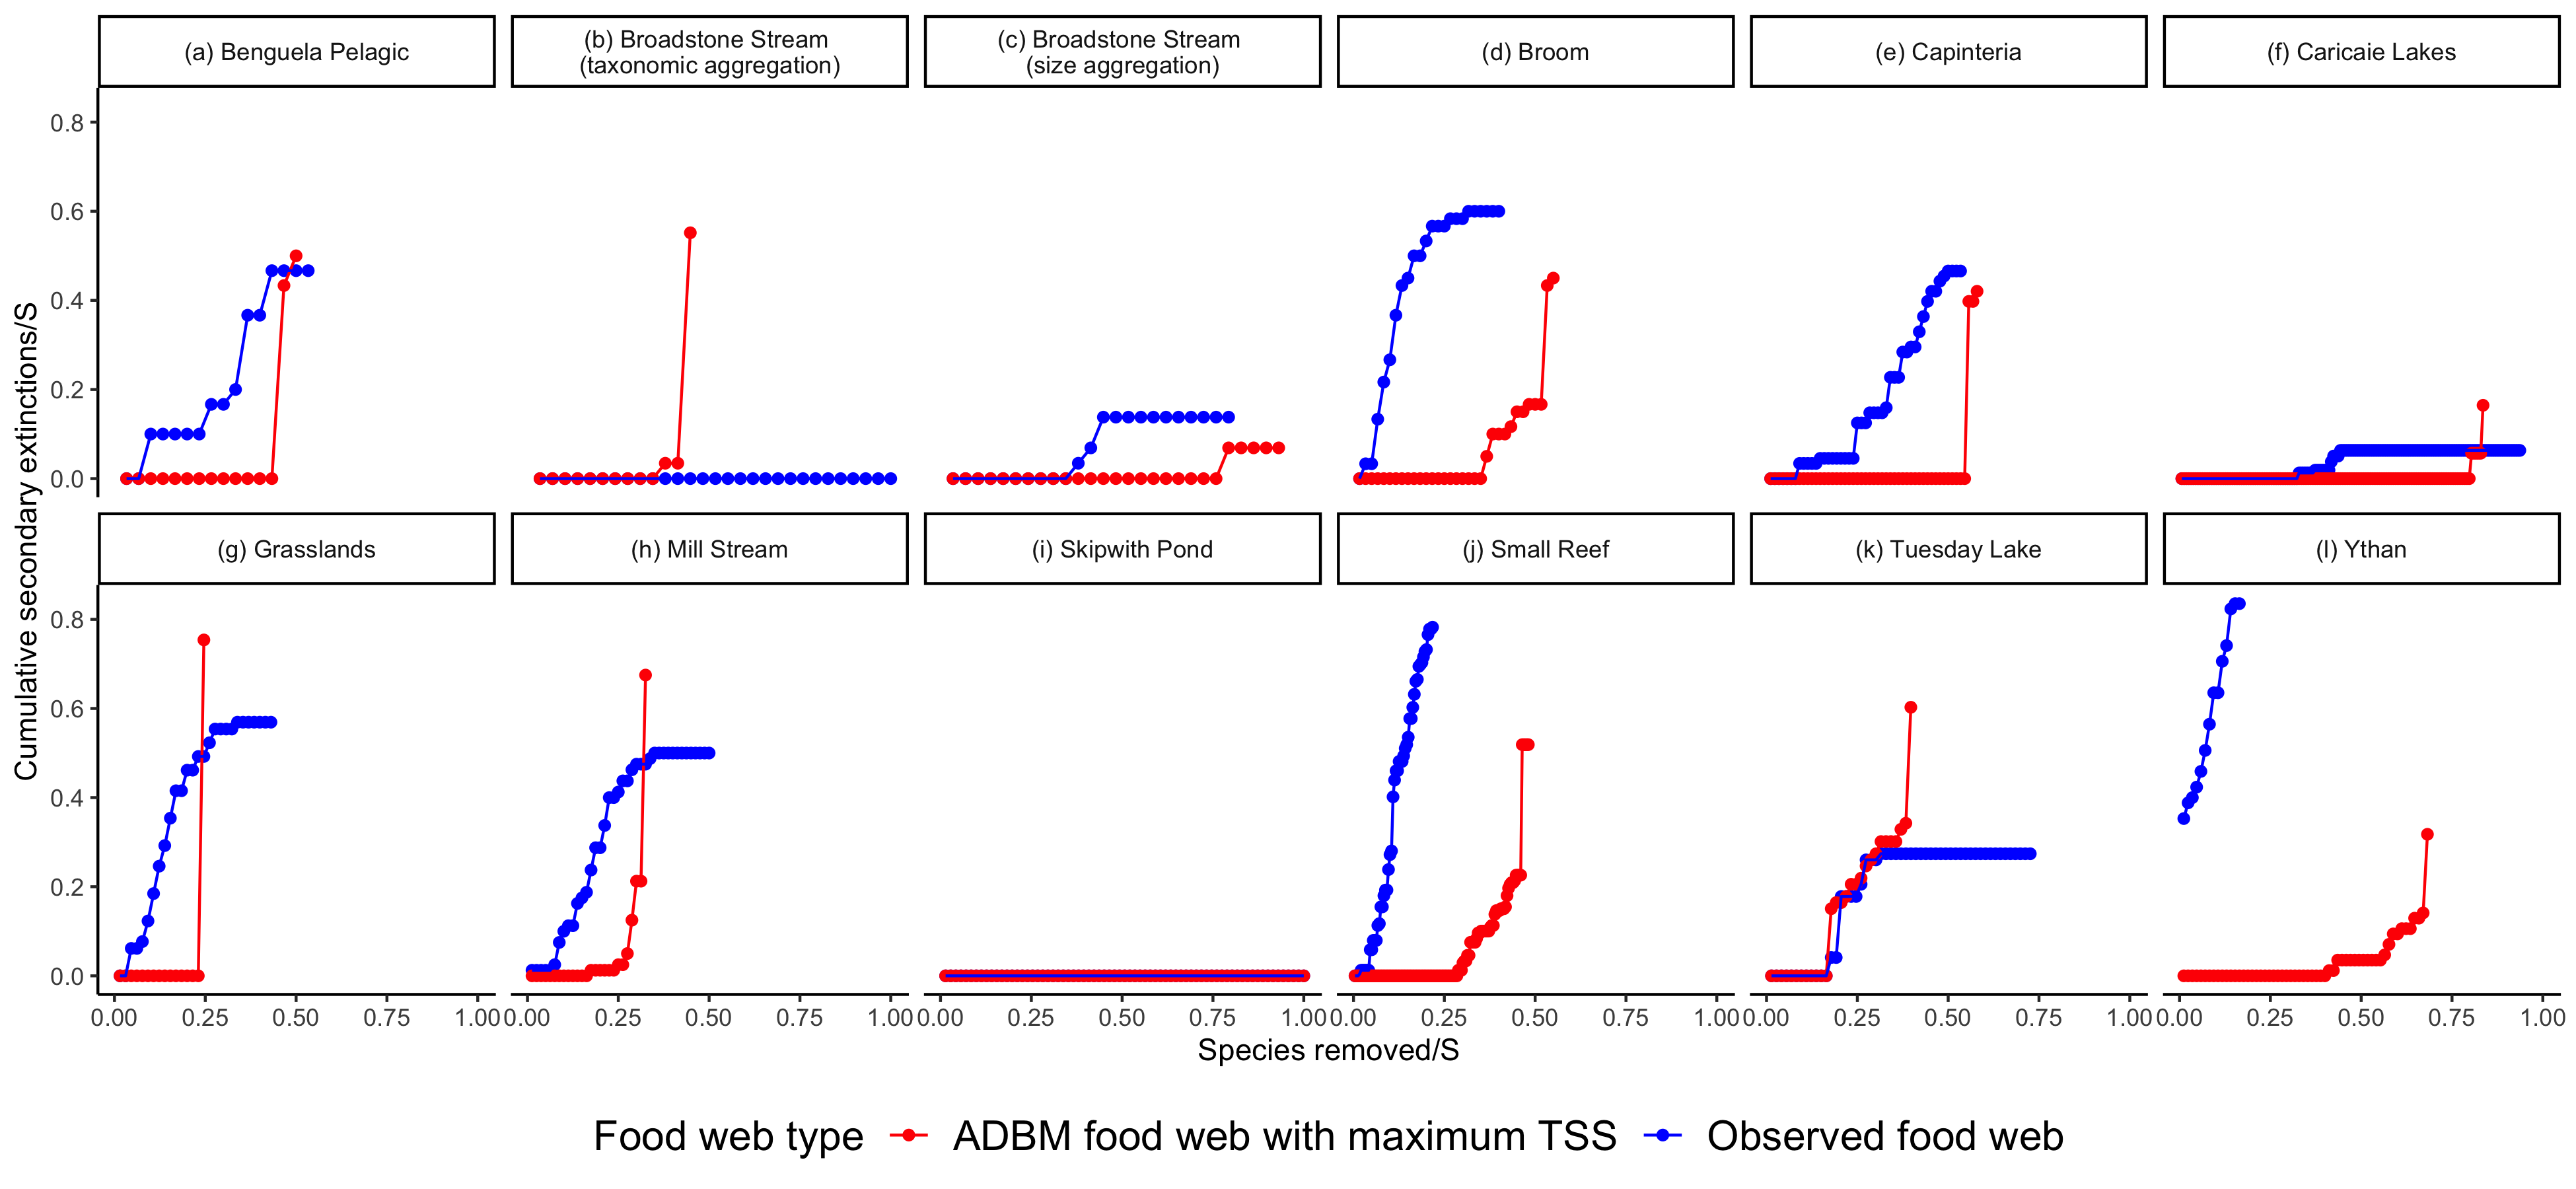
\includegraphics[width=400px]{../results/plot_mostconnected_maxTSS} 

}

\caption{\label{fig:fig_r1} Cumulative secondary extinctions of species resulting from the primary \textbf{removals of the most connected species} in the ADBM predicted food webs corresponding to the maximum TSS and observed food webs. S denotes the number of species in a food web. The cumulative secondary extinctions of species and the number of species removed have been normalised by the number of species.}\label{fig:unnamed-chunk-2}
\end{figure}

In Fig. \ref{fig:fig_r2}, we present the cumulative secondary
extinctions in the ADBM predicted and the observed food webs for five
(out of 1000) independent random extinction sequences to show
qualitative differences between their secondary extinction curves. The
secondary extinctions in the ADBM predicted food webs were more abrupt
than that in the observed food webs.

\begin{figure}

{\centering 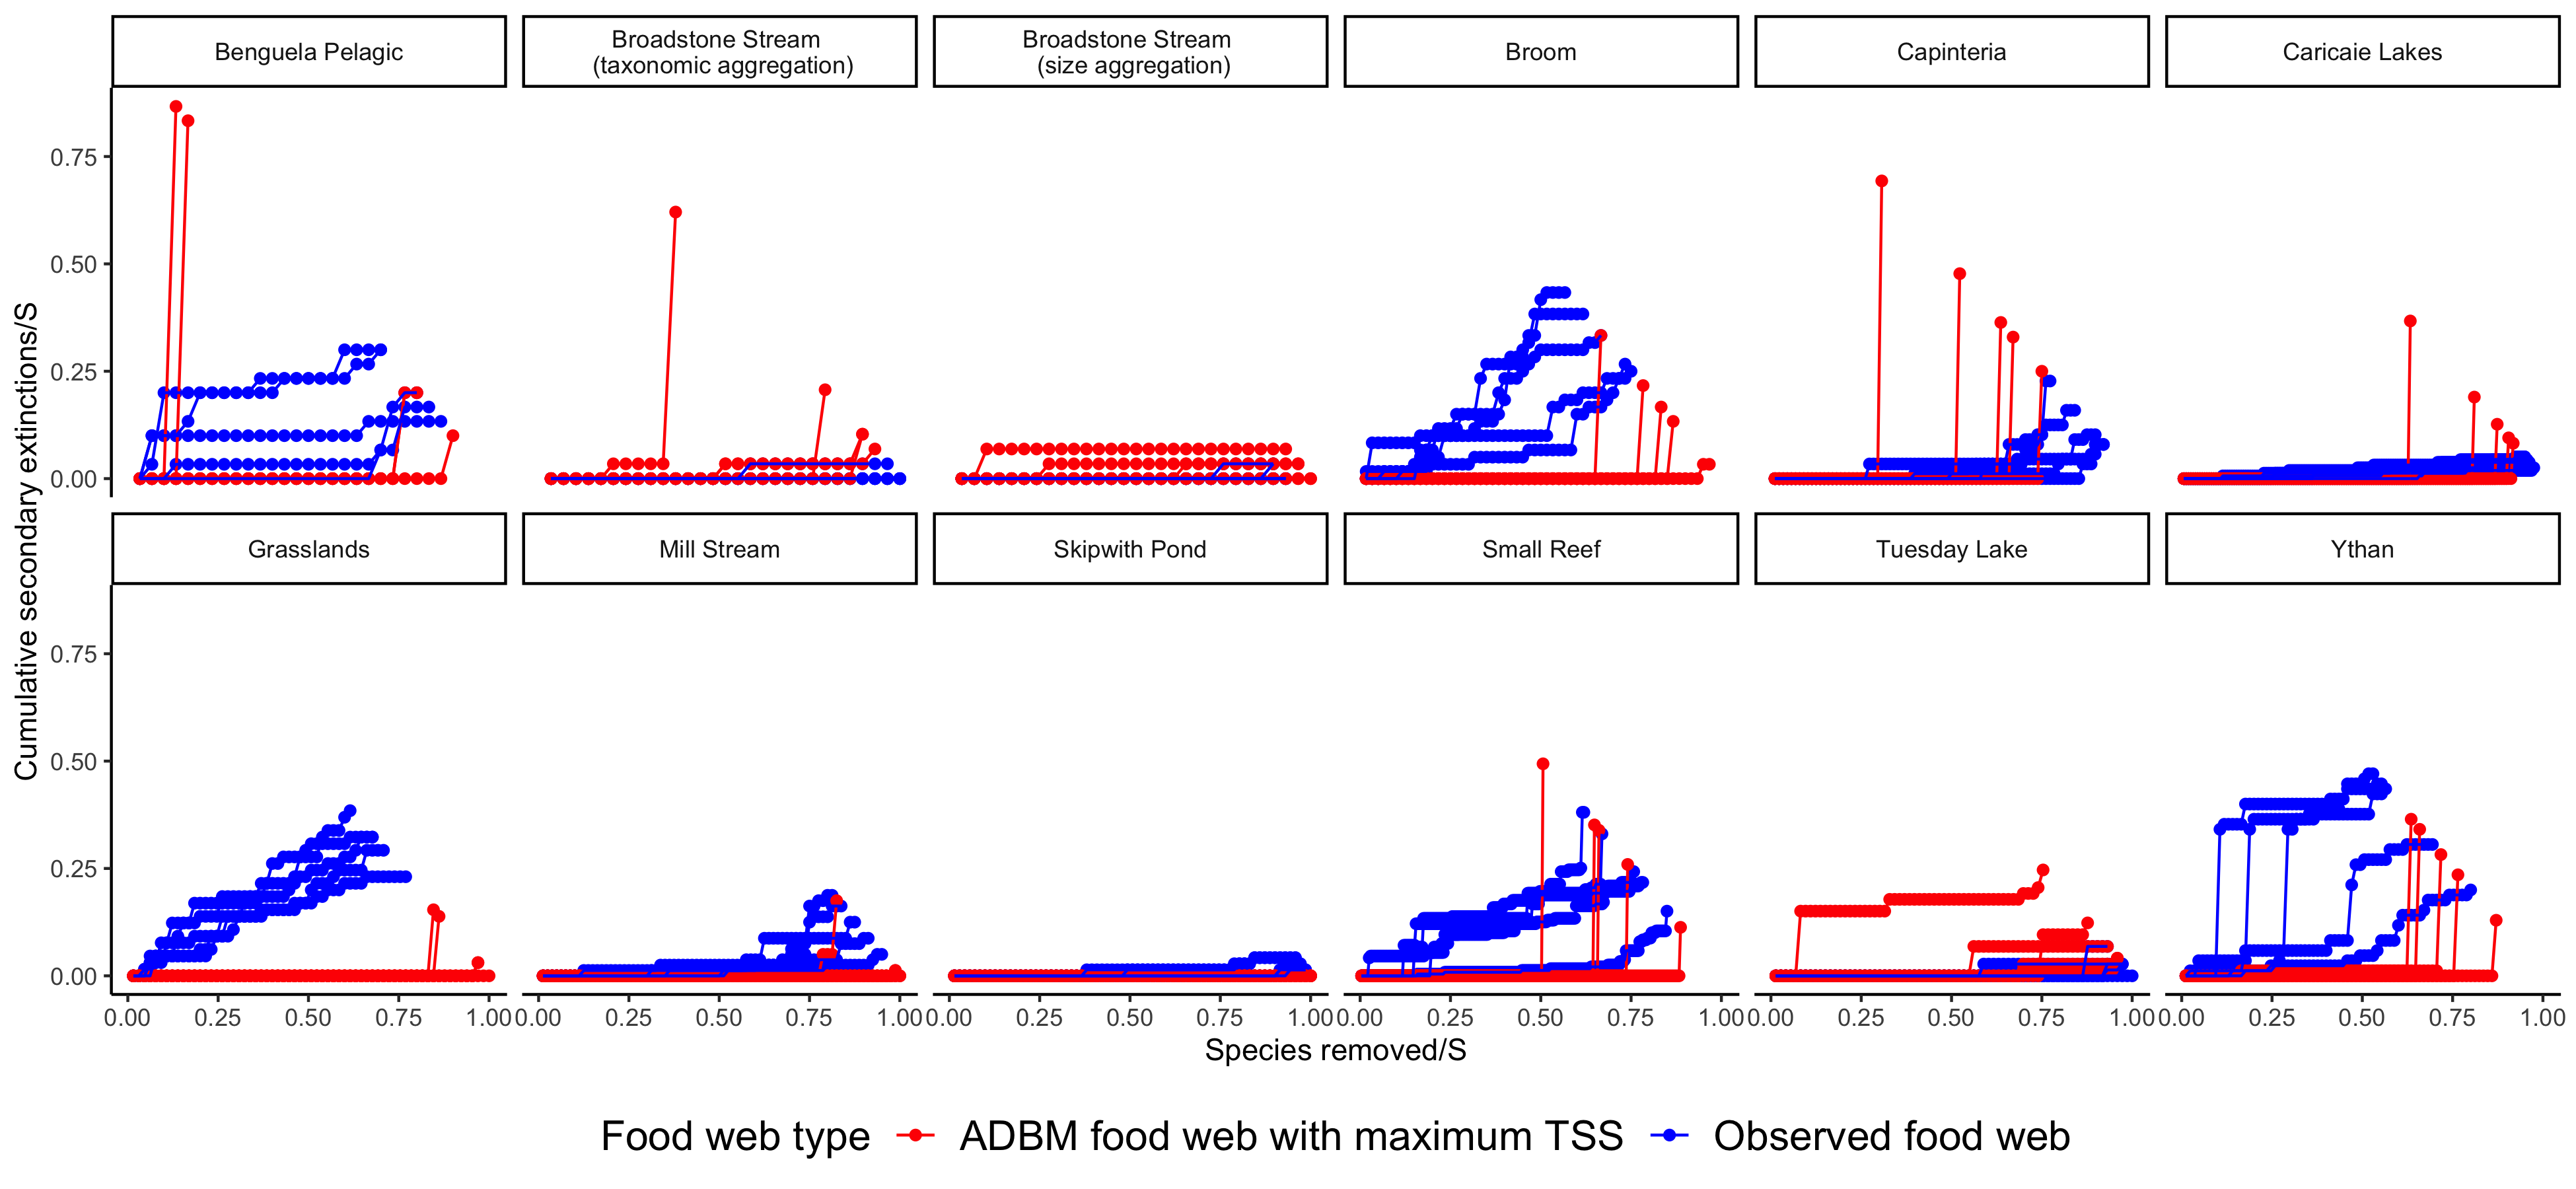
\includegraphics[width=400px]{../results/plot_ra_extlines_maxTSS} 

}

\caption{\label{fig:fig_r2} Cumulative secondary extinctions of species resulting from the primary \textbf{removals of random species} in the ADBM predicted food webs corresponding to the maximum TSS and observed food webs for five independent random extinction sequences. S denotes the number of species in a food web. The cumulative secondary extinctions of species and the number of species removed have been normalised by the number of species.}\label{fig:unnamed-chunk-3}
\end{figure}

Compared to the most-connected and random extinction scenarios, there
were fewer secondary extinctions in the least-connected extinction
scenario and therefore the secondary extinction curves were flat for
most of the food webs (Fig. \ref{fig:fig_r3}). In some of the food webs,
the extinction curves of the ADBM predicted food webs overlapped with
the observed food webs (Fig. \ref{fig:fig_r3} (b, c, g, h, i, k, l)\}).
Contrary to the most-connected scenario, there was a very high number of
secondary extinctions occurring at very low number of primary species
removal (Fig. \ref{fig:fig_r3} (a, d, e, f, j)).

\begin{figure}

{\centering 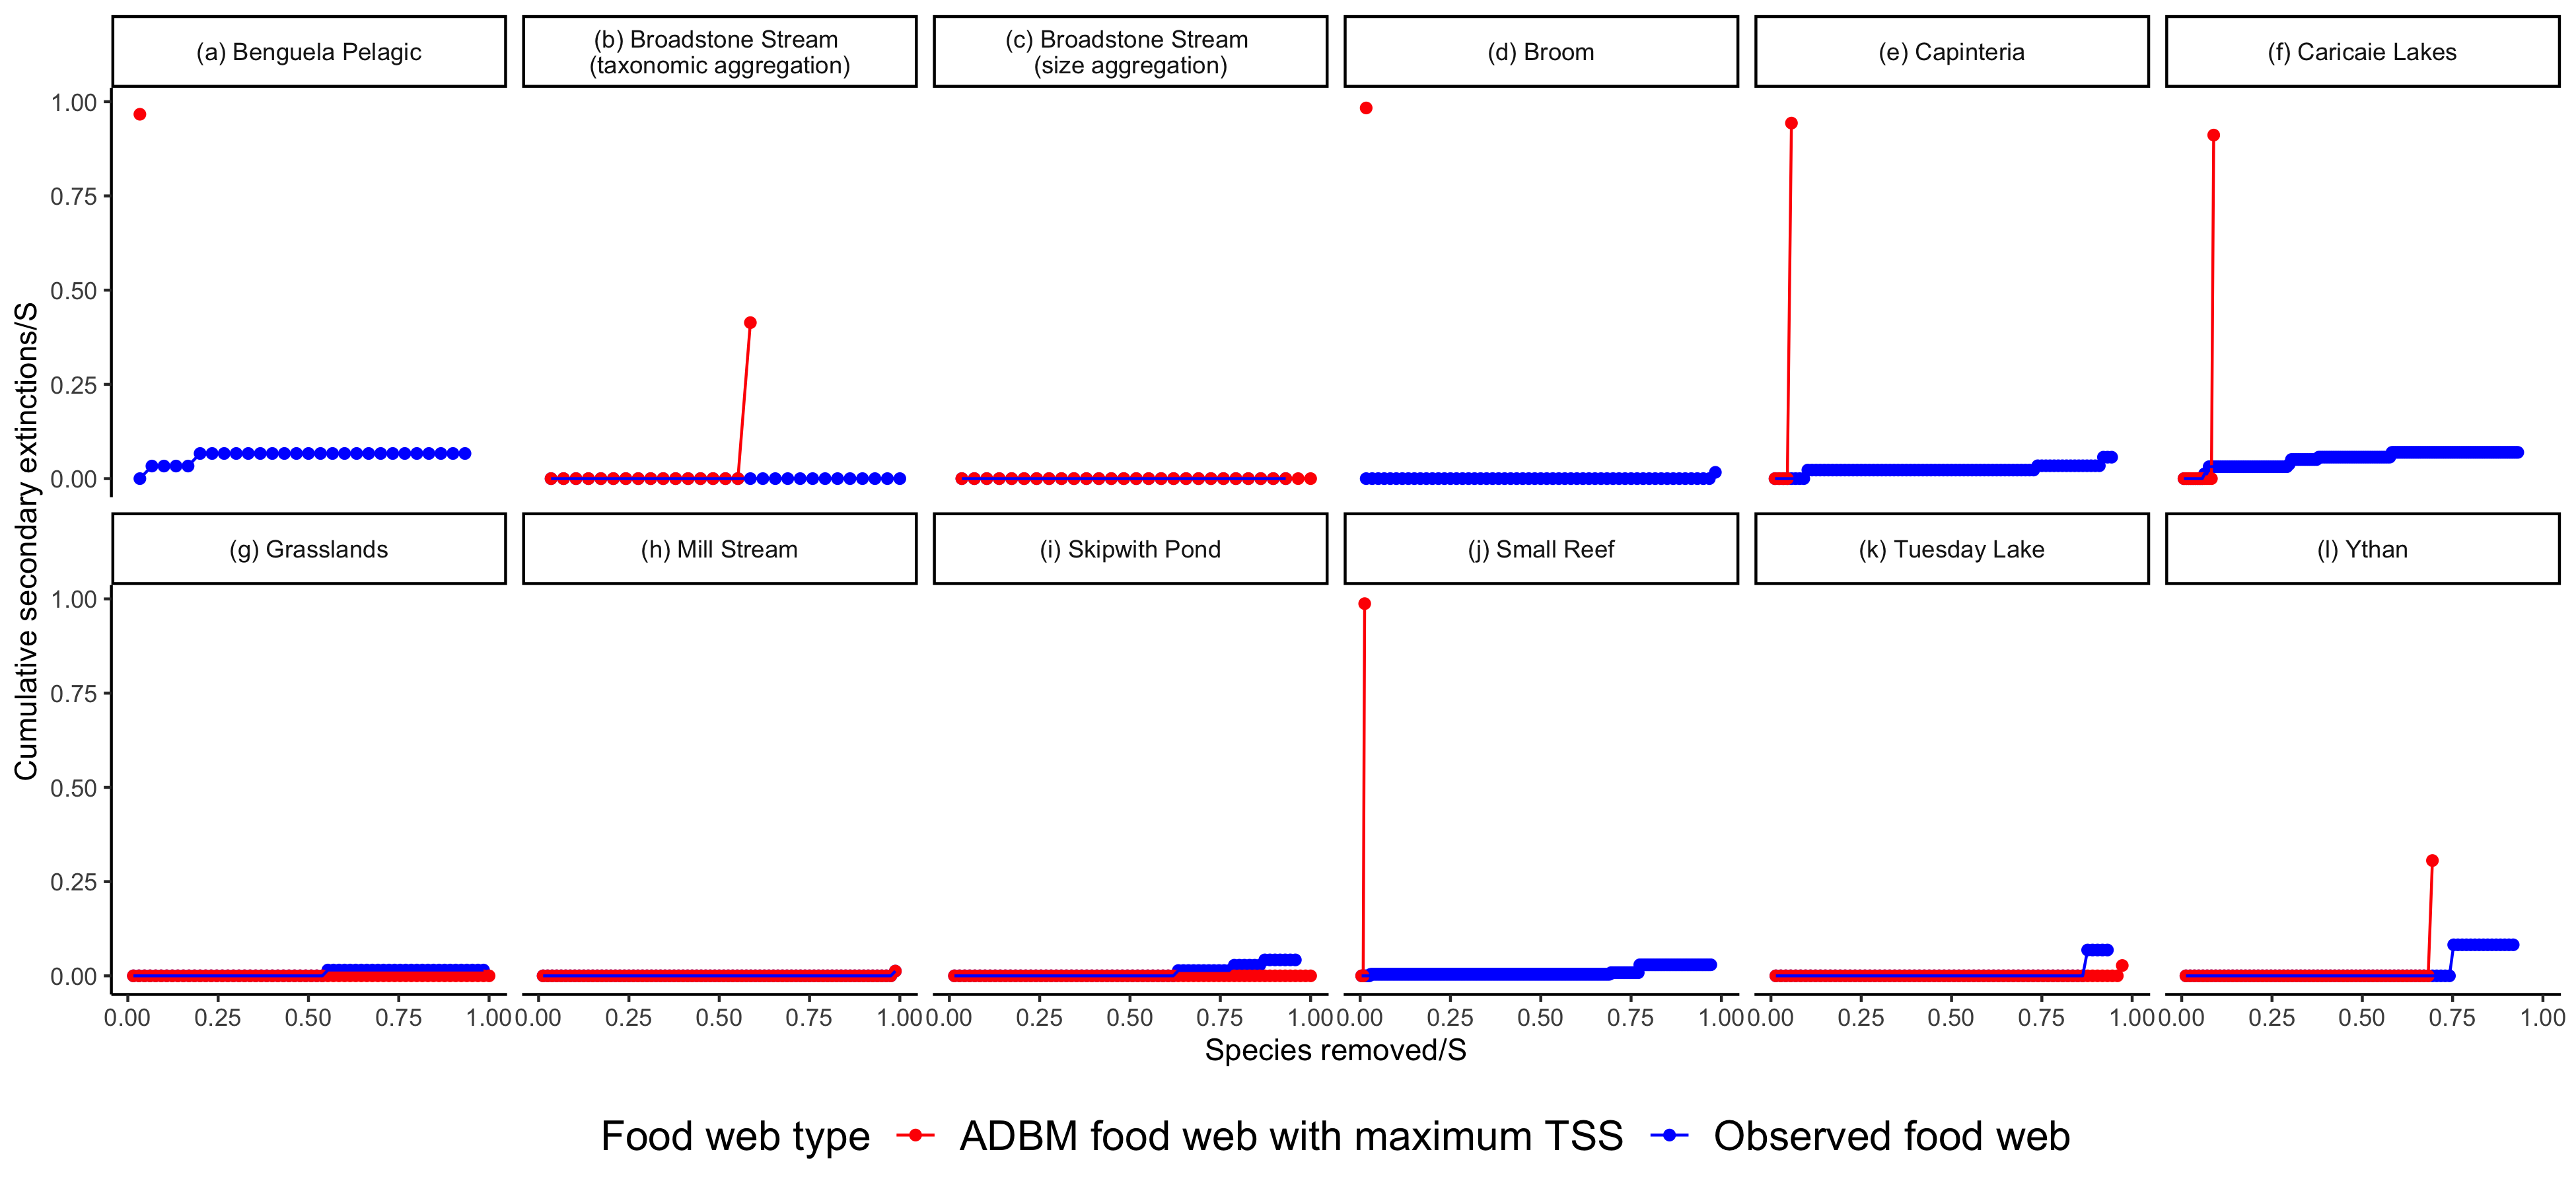
\includegraphics[width=400px]{../results/plot_leastconnected_maxTSS} 

}

\caption{\label{fig:fig_r3} Cumulative secondary extinctions of species resulting from the primary \textbf{removals of the least connected species} in the ADBM predicted food webs corresponding to the maximum TSS and observed food webs. S denotes the number of species in a food web. The cumulative secondary extinctions of species and the number of species removed have been normalised by the number of species.}\label{fig:unnamed-chunk-4}
\end{figure}

\hypertarget{robustness}{%
\subsection{Robustness}\label{robustness}}

The ADBM predicted food webs were more robust than the observed food
webs on average in the most-connected and random extinction scenarios
(Fig. \ref{fig:fig_r4} (a, b)). However, there were large variations in
the robustness within the ADBM predicted food webs in the most-connected
extinction scenario (Fig. \ref{fig:fig_r4} (a)). For example, the ADBM
predicted Caricaie Lakes food web was more robust than the observed food
web on average but had a larger variation in the robustness within the
ADBM predicted food webs compared to other food webs.

The food webs were more robust to the random extinction scenario than
the most-connected scenario (Fig. \ref{fig:fig_r4} (a, b)). Small Reef
and Benguela Pelagic food webs had more variations in robustness within
the ADBM predicted food webs as compared to the other food webs (Fig.
\ref{fig:fig_r4} (b)). Skipwith Pond, Broadstone Stream (taxonomic
aggregation) and Broadstone Stream (size aggregation) food webs were the
most robust (Median \(R_{50} = 0.5\)) for both ADBM predicted and
observed food webs. Although there were few less robust ADBM predicted
food webs in the Broadstone Stream (size aggregation) as shown by the
outliers.

In the least-connected extinction scenario, the food webs had a very
high robustness (Median \(R_{50} = 0.5\)) for most of the food webs
(Fig. \ref{fig:fig_r4} (c)), however there were some exceptions. The
ADBM predicted food webs for Small Reef and Benguela Pelagic had very
low median robustness. Benguela Pelagic, Broom and Capinteria food webs
from the ADBM had larger variations in robustness when compared to that
of the others.

\begin{figure}

{\centering 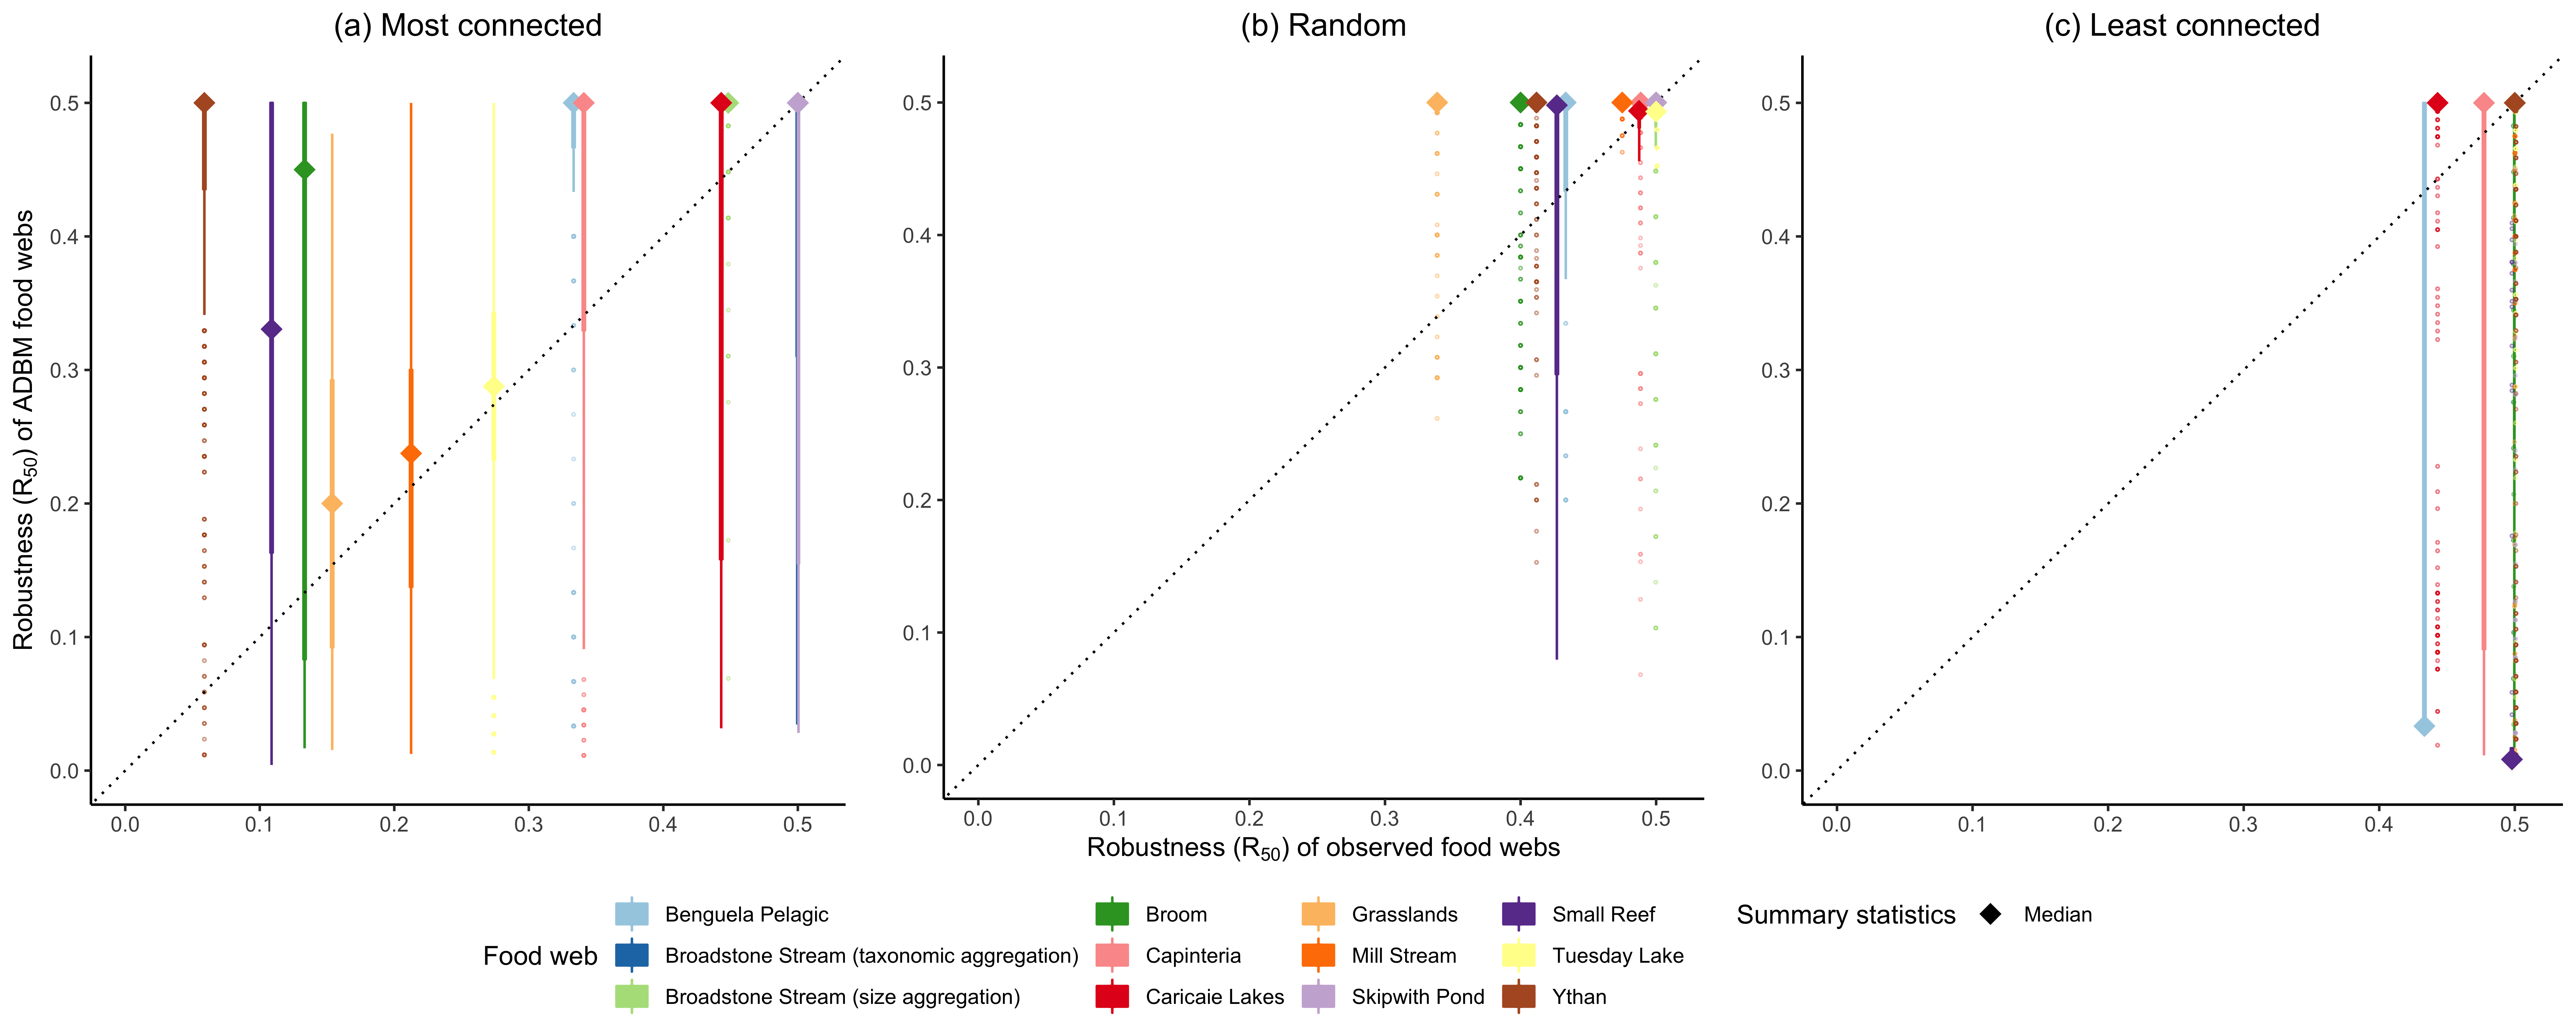
\includegraphics[width=450px]{../results/plot_R50_ADBM_vs_obs} 

}

\caption{\label{fig:fig_r4} Robustness comparison between the ADBM predicted food webs and the observed food webs for 12 food webs across different ecosystems. Here, $R_{50}$ is the proportion of species that have to be removed to achieve a total loss of at least 50\% of total species (primary removals and secondary extinctions). Box represent 25th and 75th percentile; solid diamond represent median; whisker represent outlier limits; the outlier coefficient used was 1.5. Some points are not visible due to perfect overlap in b and c. Refer to Fig. 7 in the Supplementary Information for a faceted visualisation.}\label{fig:unnamed-chunk-5}
\end{figure}

In all of the food webs except Small Reef and Broadstone Stream
(taxonomic aggregation), the effect size was positive on average in the
most-connected extinction scenario (Fig. \ref{fig:fig_r5} (a))
i.e.~overestimation of connectance had a positive effect on the
robustness. In the random extinction scenario, there was a positive
effect of overestimation of connectance on the robustness for Ythan,
Small Reef, Mill Stream, Grasslands, Caricaie Lakes, Capinteria, Broom
and Benguela Pelagic (Fig. \ref{fig:fig_r5} (b)). However, the effect
size varied across the food webs. In the least-connected extinction
scenario, the overestimation of connectance had little effect on average
on the difference in the robustness (Fig. \ref{fig:fig_r5} (c)).

\begin{figure}

{\centering 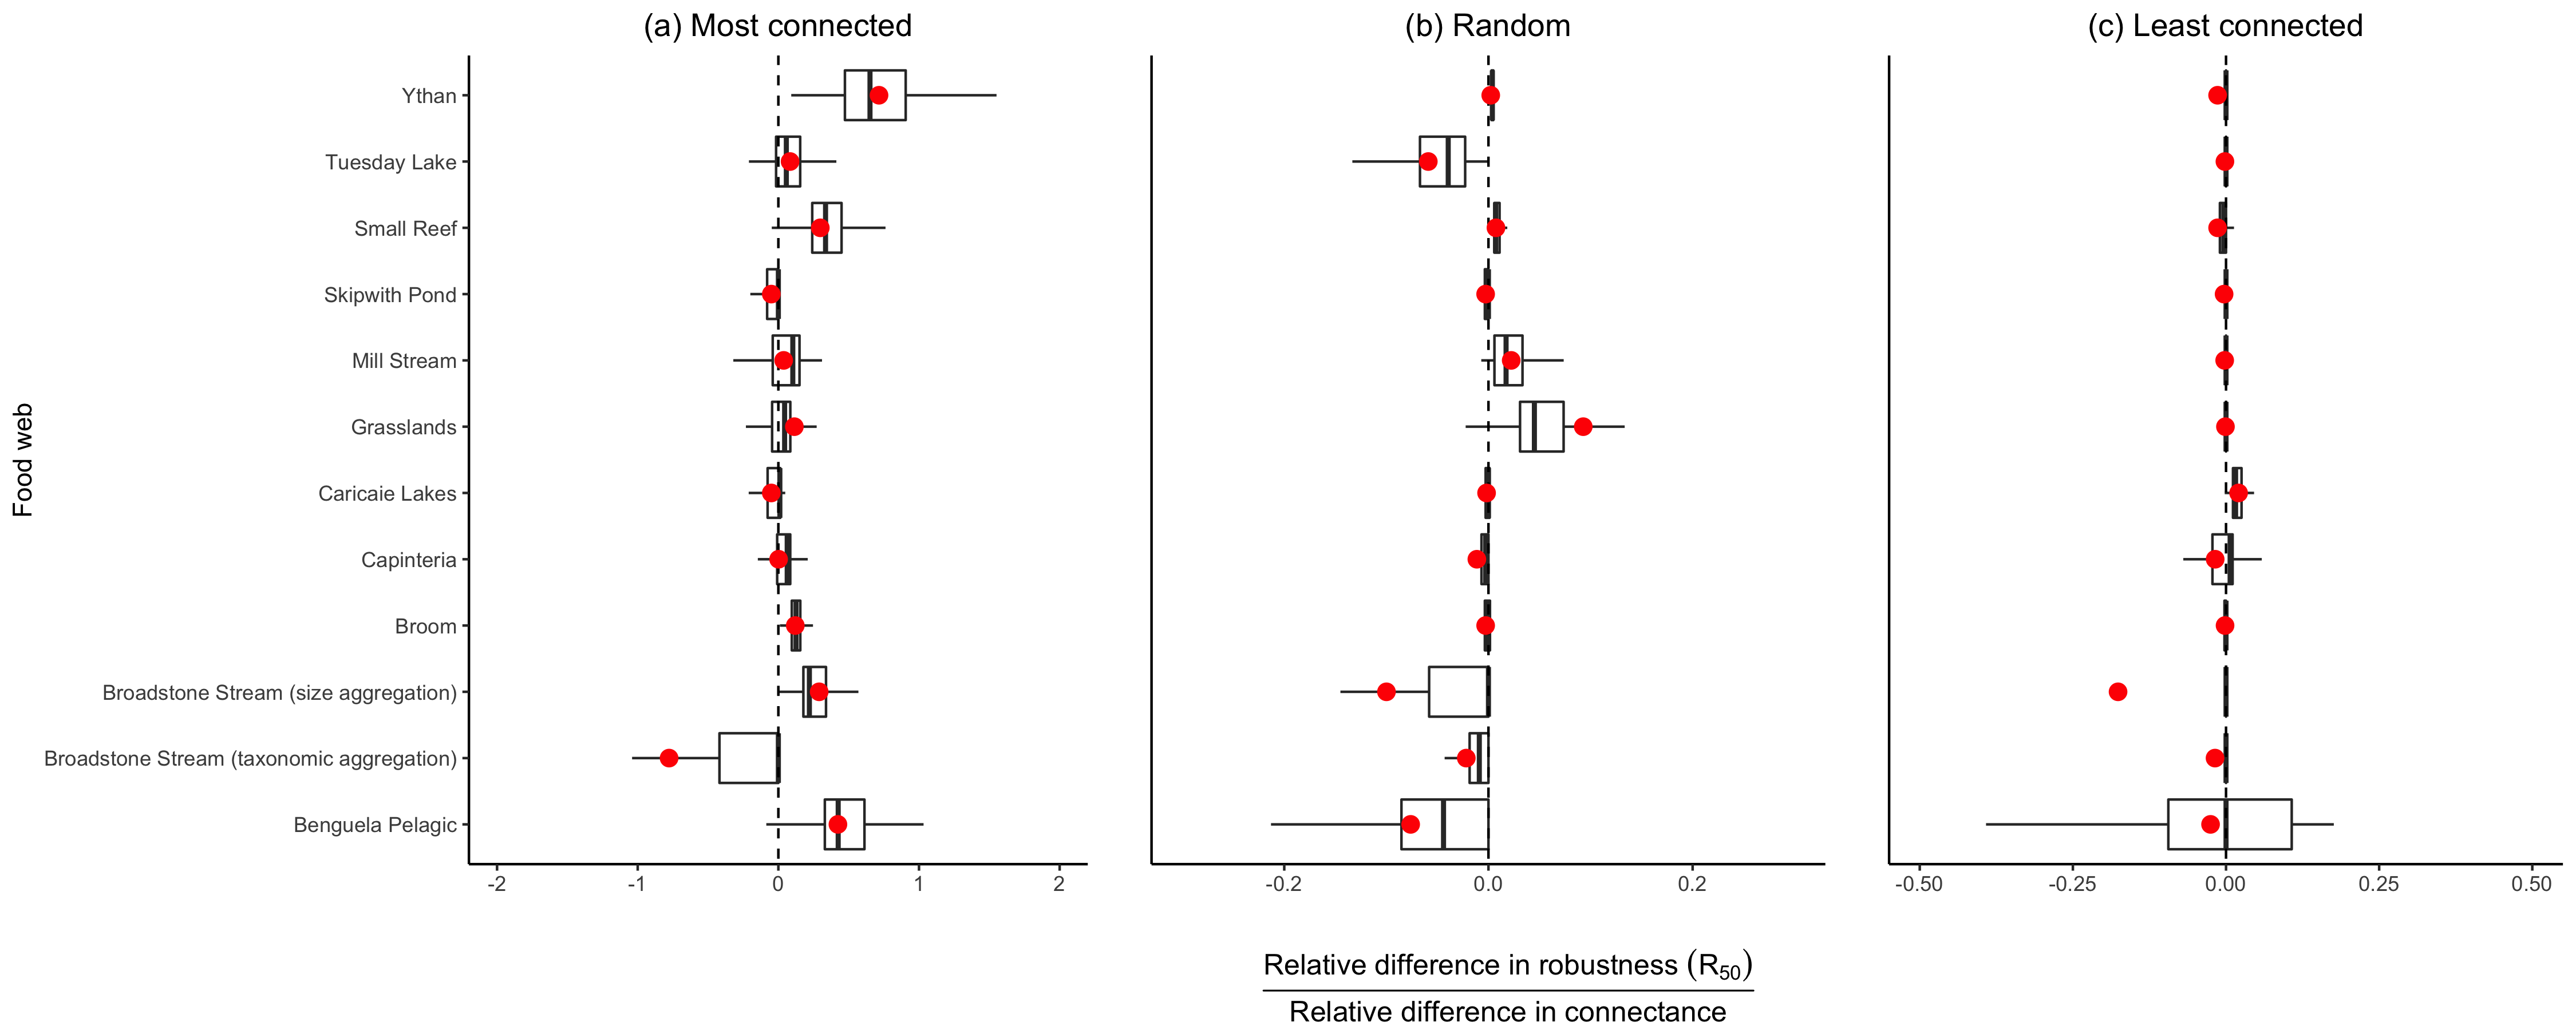
\includegraphics[width=450px]{../results/plot_R50_slope} 

}

\caption{\label{fig:fig_r5} Effect size (i.e ratio of difference in normalised robustness between ADBM predicted food webs and observed food webs to difference in their normalised connectance) shown for the 12 food webs. Box represent 25th and 75th percentile; black bold midline represent median; whisker represent outlier limits; the outlier coefficient used was 1.5.}\label{fig:unnamed-chunk-6}
\end{figure}

\hypertarget{discussion}{%
\section{Discussion}\label{discussion}}

The primary removal of species revealed that the ADBM predicted food
webs are more robust than the observed food webs on average, with
variation within the robustness of the ADBM predicted food webs in the
12 food web ecosystems suggesting that undersampling in food webs can
lead to differences in the estimates of food web robustness. The food
webs are least robust to primary extinction of the most connected
species scenario compared to that of least connected and random
extinction scenarios on average. A future development would be to
understand how undersampling i.e.~overestimation of connectance
influences the stability of the dynamics of the ADBM predicted food webs
against that of the observed food webs, and compare it with our study.

The robustness of the ADBM predicted food webs were higher than that of
the observed food webs on average (Fig. \ref{fig:fig_r4}) for all of the
12 food web ecosystems with some exceptions. This can be attributed to
the higher connectance of the ADBM predicted food webs as compared to
that of the observed food webs because a species in a food web with a
higher connectance has on average more trophic links as compared to a
food web with a lower connectance (Fig. \ref{fig:fig_r5}). Our study
suggests that it is important to consider undersampling in observed food
webs when computing their robustness.

The findings from our study are similar to what had been documented for
other food web models (Jennifer A. Dunne and Williams 2009), in terms of
an increase in the robustness when the connectance of a food web is
increased. However, contrary to general expectations (Jennifer A. Dunne,
Williams, and Martinez 2002a), food web robustness did not always
increase with the connectance (Fig. \ref{fig:fig_r5}). The ADBM
consistently predicted higher connectance than that of the observed food
webs however, in some cases an increase in connectance resulted in lower
robustness (Fig. \ref{fig:fig_r5}) in the predicted food web. For
example: the Benguela Pelagic and Small Reef food webs were surprisingly
less robust to primary extinctions on average in the least-connected
extinction scenario (Fig. \ref{fig:fig_r4} (c) and \ref{fig:fig_r5}
(c)). We suspect this is because the ADBM is underestimating the
proportion of basal species in the predicted food webs when compared to
that of the observed food webs (Fig: 6 (a) in Gupta, Furrer, and Petchey
(2022)). As a result, these low degree basal species are the ones to be
removed at an early stage in the deletion sequence thereby resulting in
an earlier food web collapse in the ADBM predicted food web as compared
to that of the observed food web (Fig: \ref{fig:fig_r3} (a) and (j)).
This suggests that the overestimation of connectance by the ADBM
resulted in a more robust food web on average but differences in the
predicted food web properties such as underestimation of the proportion
of basal species and overestimation of the maximum trophic level (Fig:
\ref{fig:fig_a1}) counteracted that effect and led to reduced
robustness. This suggests that food web properties other than
connectance play an important role in determining the robustness of a
food web and therefore should be also taken into account.

The ADBM based on its size-based rules predicts the diet of a consumer
and hence is able to predict some links in the predicted food webs which
do in reality occur but are actually not observed in the observed food
webs perhaps because of low sampling effort. A future study could be to
extend our study to use other food webs models based on size-based rules
such as Gravel et al. (2013) and Vagnon et al. (2021) and compare them
with our study. We expect similar results because these food webs are
also based on body size rules.

As with any food web model, we expect that there are real false
positives in the food webs predicted by the ADBM. Firstly this may be
because the ADBM uses only body size as a trait. A trait uncorrelated
with the body size may be influential in determining the interaction
between two species (Gupta, Furrer, and Petchey 2022). Secondly, the
ADBM can only predict diets that are contiguous with respect to the size
of the prey. I.e. it cannot predict that the consumer will consume prey
of size 1 and 3, and not consume prey of size 2. However, it is
important to note that observed diets are not always contiguous when
prey are ordered by their size due to some ecological differences in how
predator species choose their prey (Caron et al. 2022). Therefore a
future study could extend our study with other food web models which are
not based on body size such as Cattin et al. (2004) and Allesina,
Alonso, and Pascual (2008). We expect to have a difference in results
based on whether the trophic interactions in the food webs are governed
by size-structured rules or not.

It would be intriguing to know if this difference in connectance has a
similar influence on the dynamical stability of the food webs as well.
Hence, a prospect could be to use a dynamical model (for example
bioenergetic food web model by Brose, Williams, and Martinez (2006)) to
model the temporal dynamics of the ADBM predicted food webs. We expect
that the difference in dynamical robustness of the ADBM predicted and
the observed food webs would be similar to differences in their
topological robustness because the dynamical robustness of the ADBM
predicted and the observed food webs would be both underestimated when
compared to their topological robustness (Curtsdotter et al. 2011).

Since the ADBM underestimates the proportion of basal species and
overestimates the maximum trophic level in the predicted food webs
compared to that of the observed food webs, it would be interesting to
use these properties as summary statistics to parameterise the ADBM and
investigate how that influences the difference in the robustness between
the ADBM predicted and the observed food webs.

We have used a food web model to compensate for undersampling in
recorded food webs and thereby quantified the influence of missing links
i.e.~overestimation of connectance on the topological robustness of 12
food webs from various ecosystems. We found that the overestimation of
connectance can have large impacts on the robustness of the food webs
with variation in robustness among the predicted food webs which have
also been influenced by differences in the structural food web
properties between the ADBM predicted food webs and the observed food
webs.

\hypertarget{acknowledgements}{%
\section{Acknowledgements}\label{acknowledgements}}

This work was supported by the University Research Priority Program
Global Change and Biodiversity (Grant number: U-704-04-11) of the
University of Zurich.

\hypertarget{conflict-of-interest}{%
\section{Conflict of interest}\label{conflict-of-interest}}

None declared

\hypertarget{author-contributions}{%
\section{Author contributions}\label{author-contributions}}

\textbf{Anubhav Gupta:} Conceptualisation; Data curation; Formal
analysis; Investigation; Methodology; Project administration; Software;
Validation; Writing -- original draft; Writing -- review and editing.
\textbf{Owen L. Petchey:} \textbf{AG:} Owen, Could you please add your
contributions here?

\hypertarget{data-accessibility-statement}{%
\section{Data Accessibility
Statement}\label{data-accessibility-statement}}

To be added

\hypertarget{supplementary-information}{%
\section{Supplementary Information}\label{supplementary-information}}

\begin{figure}

{\centering 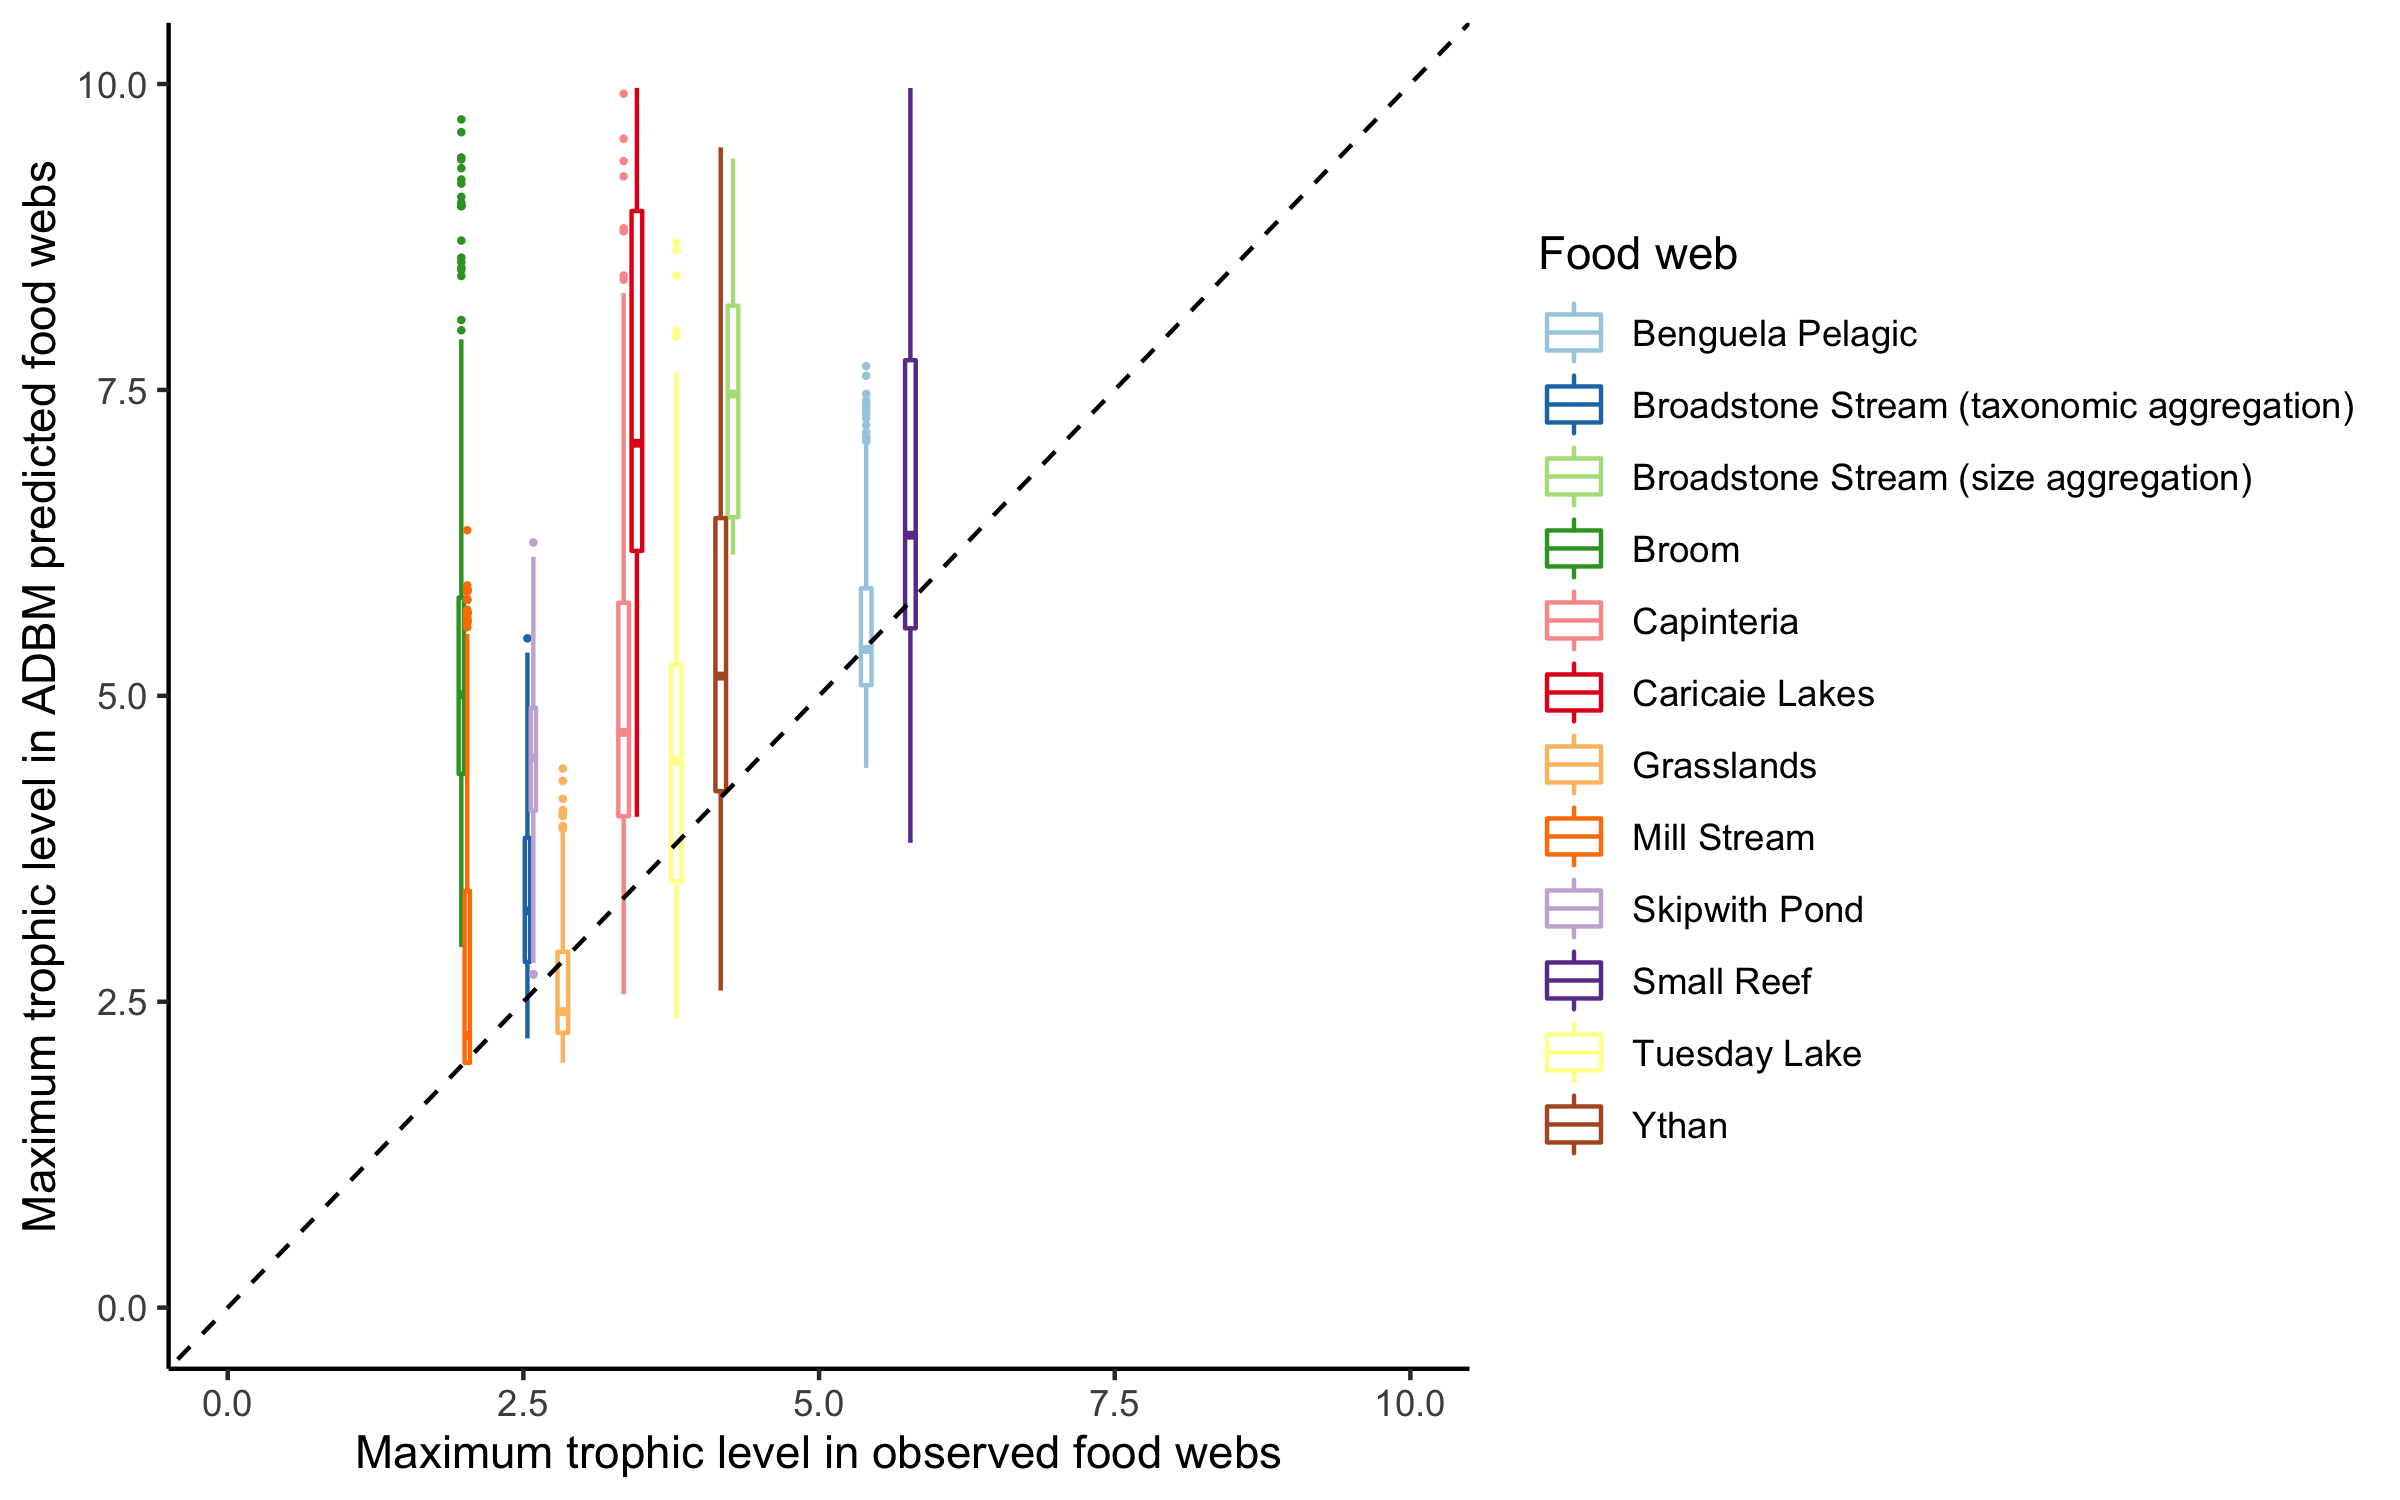
\includegraphics[width=450px]{../results/plot_max_tl_ADBM_vs_emp} 

}

\caption{\label{fig:fig_a1} Maximum trophic level of ADBM predicted food webs plotted against that of the observed food webs. Box represent 25th and 75th percentile; bold midline represent median; whisker represent outlier limits; the outlier coefficient used was 1.5.}\label{fig:unnamed-chunk-7}
\end{figure}

\begin{figure}

{\centering 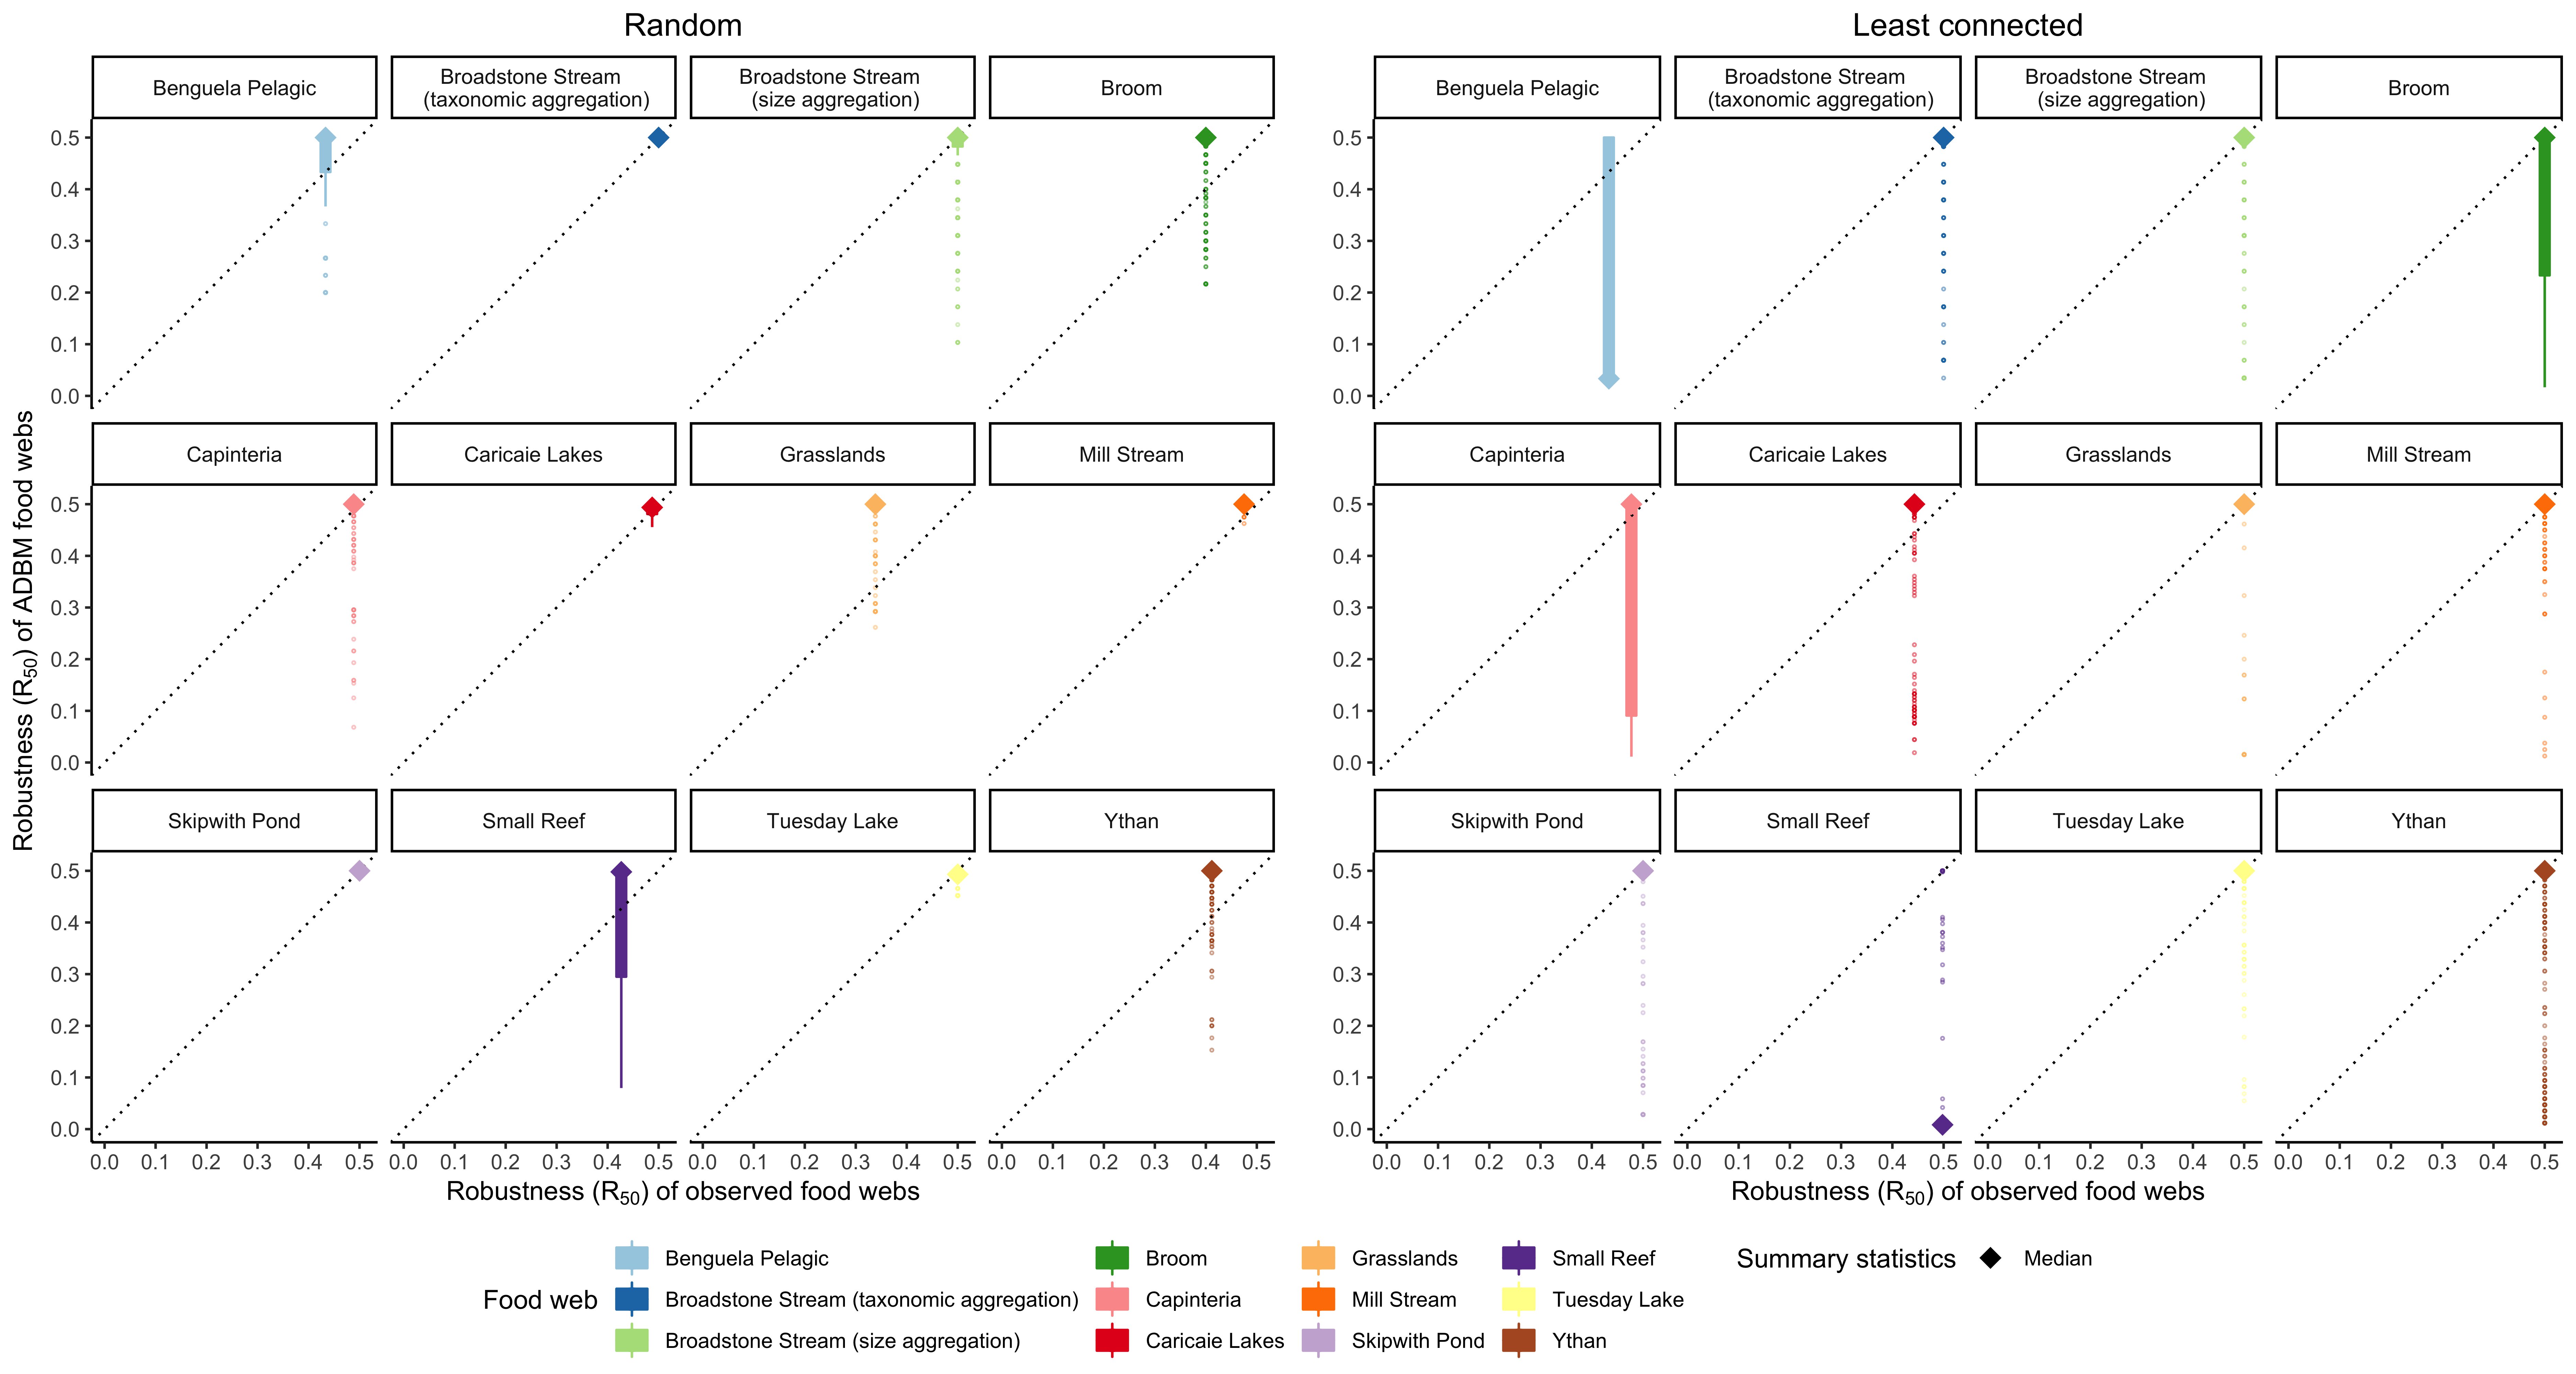
\includegraphics[width=450px]{../results/plot_R50_ADBM_vs_obs_ra_lc_facet} 

}

\caption{\label{fig:fig_a2} Robustness comparison between the ADBM predicted food webs and the observed food webs for 12 food webs across different ecosystems for random and least connected extinction scenarios. Here, $R_{50}$ is the proportion of species that have to be removed to achieve a total loss of at least 50\% of total species (primary removals and secondary extinctions). Box represent 25th and 75th percentile; solid diamond represent median; whisker represent outlier limits; the outlier coefficient used was 1.5.}\label{fig:unnamed-chunk-8}
\end{figure}

\hypertarget{references}{%
\section*{References}\label{references}}
\addcontentsline{toc}{section}{References}

\hypertarget{refs}{}
\begin{CSLReferences}{1}{0}
\leavevmode\vadjust pre{\hypertarget{ref-albertStatisticalMechanicsComplex2002}{}}%
Albert, R'eka, and Albert-L'aszl'o Barab'asi. 2002. {``Statistical
Mechanics of Complex Networks.''} \emph{Reviews of Modern Physics} 74
(1): 47--97. \url{https://doi.org/10.1103/RevModPhys.74.47}.

\leavevmode\vadjust pre{\hypertarget{ref-allesinaGeneralModelFood2008}{}}%
Allesina, Stefano, David Alonso, and Mercedes Pascual. 2008. {``A
{General Model} for {Food Web Structure}.''} \emph{Science} 320 (5876):
658--61. \url{https://doi.org/10.1126/science.1156269}.

\leavevmode\vadjust pre{\hypertarget{ref-bergUsingSensitivityAnalysis2011}{}}%
Berg, Sofia, Maria Christianou, Tomas Jonsson, and Bo Ebenman. 2011.
{``Using Sensitivity Analysis to Identify Keystone Species and Keystone
Links in Size-Based Food Webs.''} \emph{Oikos} 120 (4): 510--19.
\url{https://doi.org/10.1111/j.1600-0706.2010.18864.x}.

\leavevmode\vadjust pre{\hypertarget{ref-broseAllometricScalingEnhances2006}{}}%
Brose, Ulrich, Richard J. Williams, and Neo D. Martinez. 2006.
{``Allometric Scaling Enhances Stability in Complex Food Webs.''}
\emph{Ecology Letters} 9 (11): 1228--36.
\url{https://doi.org/10.1111/j.1461-0248.2006.00978.x}.

\leavevmode\vadjust pre{\hypertarget{ref-caronAddressingEltonianShortfall}{}}%
Caron, Dominique, Luigi Maiorano, Wilfried Thuiller, and Laura J.
Pollock. 2022. {``Addressing the {Eltonian} Shortfall with Trait-Based
Interaction Models.''} \emph{Ecology Letters} n/a (n/a).
\url{https://doi.org/10.1111/ele.13966}.

\leavevmode\vadjust pre{\hypertarget{ref-cattinPhylogeneticConstraintsAdaptation2004}{}}%
Cattin, Marie-France, Louis-F'elix Bersier, Carolin Banašek-Richter,
Richard Baltensperger, and Jean-Pierre Gabriel. 2004. {``Phylogenetic
Constraints and Adaptation Explain Food-Web Structure.''} \emph{Nature}
427 (6977, 6977): 835--39. \url{https://doi.org/10.1038/nature02327}.

\leavevmode\vadjust pre{\hypertarget{ref-curtsdotterRobustnessSecondaryExtinctions2011a}{}}%
Curtsdotter, Alva, Amrei Binzer, Ulrich Brose, Francisco de Castro, Bo
Ebenman, Anna Eklöf, Jens O. Riede, Aaron Thierry, and Björn C. Rall.
2011. {``Robustness to Secondary Extinctions: {Comparing} Trait-Based
Sequential Deletions in Static and Dynamic Food Webs.''} \emph{Basic and
Applied Ecology} 12 (7): 571--80.
\url{https://doi.org/10.1016/j.baae.2011.09.008}.

\leavevmode\vadjust pre{\hypertarget{ref-dunne2004}{}}%
Dunne, Ja, Rj Williams, and Nd Martinez. 2004. {``Network Structure and
Robustness of Marine Food Webs.''} \emph{Marine Ecology Progress Series}
273: 291--302. \url{https://doi.org/10.3354/meps273291}.

\leavevmode\vadjust pre{\hypertarget{ref-dunneCascadingExtinctionsCommunity2009}{}}%
Dunne, Jennifer A., and Richard J. Williams. 2009. {``Cascading
Extinctions and Community Collapse in Model Food Webs.''}
\emph{Philosophical Transactions of the Royal Society B: Biological
Sciences} 364 (1524): 1711--23.
\url{https://doi.org/10.1098/rstb.2008.0219}.

\leavevmode\vadjust pre{\hypertarget{ref-dunneNetworkStructureBiodiversity2002}{}}%
Dunne, Jennifer A., Richard J. Williams, and Neo D. Martinez. 2002a.
{``Network Structure and Biodiversity Loss in Food Webs: Robustness
Increases with Connectance.''} \emph{Ecology Letters} 5 (4): 558--67.
\url{https://doi.org/10.1046/j.1461-0248.2002.00354.x}.

\leavevmode\vadjust pre{\hypertarget{ref-dunne2002network}{}}%
Dunne, Jennifer A, Richard J Williams, and Neo D Martinez. 2002b.
{``Network Structure and Biodiversity Loss in Food Webs: Robustness
Increases with Connectance.''} \emph{Ecology Letters} 5 (4): 558--67.

\leavevmode\vadjust pre{\hypertarget{ref-ebenmanUsingCommunityViability2005}{}}%
Ebenman, Bo, and Tomas Jonsson. 2005. {``Using Community Viability
Analysis to Identify Fragile Systems and Keystone Species.''}
\emph{Trends in Ecology \& Evolution} 20 (10): 568--75.
\url{https://doi.org/10.1016/j.tree.2005.06.011}.

\leavevmode\vadjust pre{\hypertarget{ref-ebenmanCOMMUNITYVIABILITYANALYSIS2004}{}}%
Ebenman, Bo, Richard Law, and Charlotte Borrvall. 2004. {``{COMMUNITY
VIABILITY ANALYSIS}: {THE RESPONSE OF ECOLOGICAL COMMUNITIES TO SPECIES
LOSS}.''} \emph{Ecology} 85 (9): 2591--2600.
\url{https://doi.org/10.1890/03-8018}.

\leavevmode\vadjust pre{\hypertarget{ref-gravelInferringFoodWeb2013a}{}}%
Gravel, Dominique, Timoth'ee Poisot, Camille Albouy, Laure Velez, and
David Mouillot. 2013. {``Inferring Food Web Structure from
Predator--Prey Body Size Relationships.''} \emph{Methods in Ecology and
Evolution} 4 (11): 1083--90.
\url{https://doi.org/10.1111/2041-210X.12103}.

\leavevmode\vadjust pre{\hypertarget{ref-guptaSimultaneouslyEstimatingFood2022}{}}%
Gupta, Anubhav, Reinhard Furrer, and Owen L. Petchey. 2022.
{``Simultaneously Estimating Food Web Connectance and Structure with
Uncertainty.''} \emph{Ecology and Evolution} 12 (3): e8643.
\url{https://doi.org/10.1002/ece3.8643}.

\leavevmode\vadjust pre{\hypertarget{ref-jonssonReliabilityR50Measure2015}{}}%
Jonsson, Tomas, Sofia Berg, Alexander Pimenov, Catherine Palmer, and
Mark Emmerson. 2015. {``The Reliability of {R50} as a Measure of
Vulnerability of Food Webs to Sequential Species Deletions.''}
\emph{Oikos} 124 (4): 446--57. \url{https://doi.org/10.1111/oik.01588}.

\leavevmode\vadjust pre{\hypertarget{ref-jordanoSamplingNetworksEcological2016}{}}%
Jordano, Pedro. 2016. {``Sampling Networks of Ecological
Interactions.''} \emph{Functional Ecology} 30 (12): 1883--93.
\url{https://doi.org/10.1111/1365-2435.12763}.

\leavevmode\vadjust pre{\hypertarget{ref-macarthur1966}{}}%
MacArthur, Robert H., and Eric R. Pianka. 1966. {``On Optimal Use of a
Patchy Environment.''} \emph{The American Naturalist} 100 (916): 603--9.
\url{https://www.jstor.org/stable/2459298}.

\leavevmode\vadjust pre{\hypertarget{ref-martinezDiversityComplexityPersistence}{}}%
Martinez, Neo D, Richard J Williams, and Jennifer A Dunne. 2006.
{``Diversity, {Complexity}, and {Persistence} in {Large Model
Ecosystems},''} 24.

\leavevmode\vadjust pre{\hypertarget{ref-patonaiAggregationIncompleteFood2017}{}}%
Patonai, Katalin, and Ferenc Jord'an. 2017. {``Aggregation of Incomplete
Food Web Data May Help to Suggest Sampling Strategies.''}
\emph{Ecological Modelling} 352 (May): 77--89.
\url{https://doi.org/10.1016/j.ecolmodel.2017.02.024}.

\leavevmode\vadjust pre{\hypertarget{ref-petchey2008}{}}%
Petchey, Owen L., A. P. Beckerman, J. O. Riede, and P. H. Warren. 2008.
{``Size, Foraging, and Food Web Structure.''} \emph{Proceedings of the
National Academy of Sciences} 105 (11): 4191--96.
\url{https://doi.org/10.1073/pnas.0710672105}.

\leavevmode\vadjust pre{\hypertarget{ref-pimmHumanImpactsRates2006}{}}%
Pimm, Stuart, Peter Raven, Alan Peterson, Çağan H. Şekercioğlu, and Paul
R. Ehrlich. 2006. {``Human Impacts on the Rates of Recent, Present, and
Future Bird Extinctions.''} \emph{Proceedings of the National Academy of
Sciences} 103 (29): 10941--46.
\url{https://doi.org/10.1073/pnas.0604181103}.

\leavevmode\vadjust pre{\hypertarget{ref-soleComplexityFragilityEcological2001}{}}%
Sol'e, Ricard V., and M. Montoya. 2001. {``Complexity and Fragility in
Ecological Networks.''} \emph{Proceedings of the Royal Society of
London. Series B: Biological Sciences} 268 (1480): 2039--45.
\url{https://doi.org/10.1098/rspb.2001.1767}.

\leavevmode\vadjust pre{\hypertarget{ref-thomasExtinctionRiskClimate2004}{}}%
Thomas, Chris D., Alison Cameron, Rhys E. Green, Michel Bakkenes, Linda
J. Beaumont, Yvonne C. Collingham, Barend F. N. Erasmus, et al. 2004.
{``Extinction Risk from Climate Change.''} \emph{Nature} 427 (6970,
6970): 145--48. \url{https://doi.org/10.1038/nature02121}.

\leavevmode\vadjust pre{\hypertarget{ref-thomasComparativeLossesBritish2004}{}}%
Thomas, J. A., M. G. Telfer, D. B. Roy, C. D. Preston, J. J. D.
Greenwood, J. Asher, R. Fox, R. T. Clarke, and J. H. Lawton. 2004.
{``Comparative {Losses} of {British Butterflies}, {Birds}, and {Plants}
and the {Global Extinction Crisis}.''} \emph{Science} 303 (5665):
1879--81. \url{https://doi.org/10.1126/science.1095046}.

\leavevmode\vadjust pre{\hypertarget{ref-ullah2018}{}}%
Ullah, Hadayet, Ivan Nagelkerken, Silvan U. Goldenberg, and Damien A.
Fordham. 2018. {``Climate Change Could Drive Marine Food Web Collapse
Through Altered Trophic Flows and Cyanobacterial Proliferation.''}
Edited by Michel Loreau. \emph{PLOS Biology} 16 (1): e2003446.
\url{https://doi.org/10.1371/journal.pbio.2003446}.

\leavevmode\vadjust pre{\hypertarget{ref-vagnonAllometricNicheModel2021}{}}%
Vagnon, Chlo'e, Franck Cattan'eo, Chlo'e Goulon, David Grimardias, Jean
Guillard, and Victor Frossard. 2021. {``An Allometric Niche Model for
Species Interactions in Temperate Freshwater Ecosystems.''}
\emph{Ecosphere} 12 (3): e03420.
\url{https://doi.org/10.1002/ecs2.3420}.

\leavevmode\vadjust pre{\hypertarget{ref-whiteEcologistsShouldNot2014}{}}%
White, J. Wilson, Andrew Rassweiler, Jameal F. Samhouri, Adrian C.
Stier, and Crow White. 2014. {``Ecologists Should Not Use Statistical
Significance Tests to Interpret Simulation Model Results.''}
\emph{Oikos} 123 (4): 385--88.
\url{https://doi.org/10.1111/j.1600-0706.2013.01073.x}.

\leavevmode\vadjust pre{\hypertarget{ref-williamsEffectsNetworkDynamical2008}{}}%
Williams, Richard J. 2008. {``Effects of Network and Dynamical Model
Structure on Species Persistence in Large Model Food Webs.''}
\emph{Theoretical Ecology} 1 (3): 141--51.
\url{https://doi.org/10.1007/s12080-008-0013-5}.

\end{CSLReferences}

\bibliographystyle{biblatex}
\bibliography{bibliography.bib}


\end{document}
